\chapter{Deep Learning the Lyman-alpha forest}
\label{chap: deep learning}




\section{Introduction and motivation for the use of Deep Learning}
\label{sec:motiv_ml}


Fundamentally, a neural network is a directed and acyclic computational graph \cite{LeCun2015}. It represents a set of operations that transform input data input an output. In the simplest case of a fully connected network, the nodes of this graph are represented by neurons. Neurons are organized on successive layers, making the information flow from a layer to the following one. In the most basic scenario, the neurons in a given layer are linearly connected to the neurons in the previous layer. Each neuron then adds a bias to the result of the computation and applies a non-linear function to the result, which determines the activation state of the neuron. Consider the graph shown in \cref{fig:MLP}, where the input neuron has a value $x$ and the output neuron has a value $y(x)$. The intermediate layers have values
\begin{equation}
    \begin{dcases}
        x_1=\sigma(\alpha_1 x+\beta_1)\\
        x_2=\sigma(\alpha_2 x+\beta_2)
    \end{dcases},
\end{equation}
where $\alpha_i$ are the linear weights, $\beta_i$ the biases, and $\sigma$ is a non-linear activation function. Typical choices include $\tanh{}$ on ReLU (Rectifier Linear Unit) given by RELu$(x)=\max(0,x)$. Graphs such as the one shown in \cref{fig:MLP} as know as \emph{fully connected layers}. Much more complex architectures have of course been investigated. Depending on the specific problem and dataset, we can incorporate a priori knowledge of the problem in the design of the network. For instance, in Computer Vision, the use of \emph{convolutional layers} especially target at identifying key features in images has proven to be extremely successful \cite{CNN_rev}. In the analysis of time series, Long short-term memory (LSTM) neurons allow the network to ``remember" information from previous inputs \cite{LSTM_rev}. 




From the theoretical standpoint, neural networks are universal approximations (for sufficiently well-behaved functions), which makes them especially appealing in the modelling of complex systems. A concrete results is as follows \cite{universal_aprox}:

\begin{theorem}[Universal approximation theorem]\label{th:aprox}

    If $f\colon \mathbb{R}^n \to \mathbb{R}^m$ is a Lebesgue p-integrable function and $\varepsilon>0$, then there exists a fully connected ReLU network $F\colon \mathbb{R}^n \to \mathbb{R}^m$ such that
    $$
        \int_{\mathbf{R}^n}||f(x)-F(x) ||^p\ \differential x <\varepsilon.
    $$
\end{theorem}
Theorem \ref{th:aprox} can be expanded to include tight bounds on the depth or width of the network, which then depend on $n$ and $m$. Note that all the complexity of a fully connected neural network is generated by the non-linear activation function. With a linear activation function, a fully connected networks would be an affine transformation, which cannot approximate arbitrary non-linear functions.

\begin{figure}
    \centering
    \begin{subfigure}[b]{0.45\textwidth}
        \centering
                    \begin{tikzpicture}[scale=0.2]


                    \node (in) [circle, fill=white, draw=black, ultra thick, minimum size=1.3cm] {$x$};
                    
                    
                    \node (neu1) [circle, fill=orange, draw=black, ultra thick, below=of in , minimum size=1.3cm, xshift=2cm] {$x_1$};
                    
                    
                    \node (neu2) [circle, fill=orange, draw=black, ultra thick, below=of in , minimum size=1.3cm, xshift=-2cm] {$x_2$};
                    
                    
                    
                    \node (out) [circle, fill=dark-cyan, draw=black, ultra thick, below=of in , minimum size=1.3cm, yshift=-2cm] {$y(x)$};
                    
                    \draw [->,ultra thick] (in) -- (neu1);
                    \draw [->,ultra thick] (in) -- (neu2);
                    \draw [->,ultra thick] (neu1) -- (out);
                    \draw [->,ultra thick] (neu2) -- (out);
                    
                    \end{tikzpicture}
        \caption{Graph for a simple MLP with a hidden layer (in orange) and an output neuron (in cyan).}
        \label{fig:MLP}
    \end{subfigure}
    \hfill
    \begin{subfigure}[b]{0.45\textwidth}
        \centering
        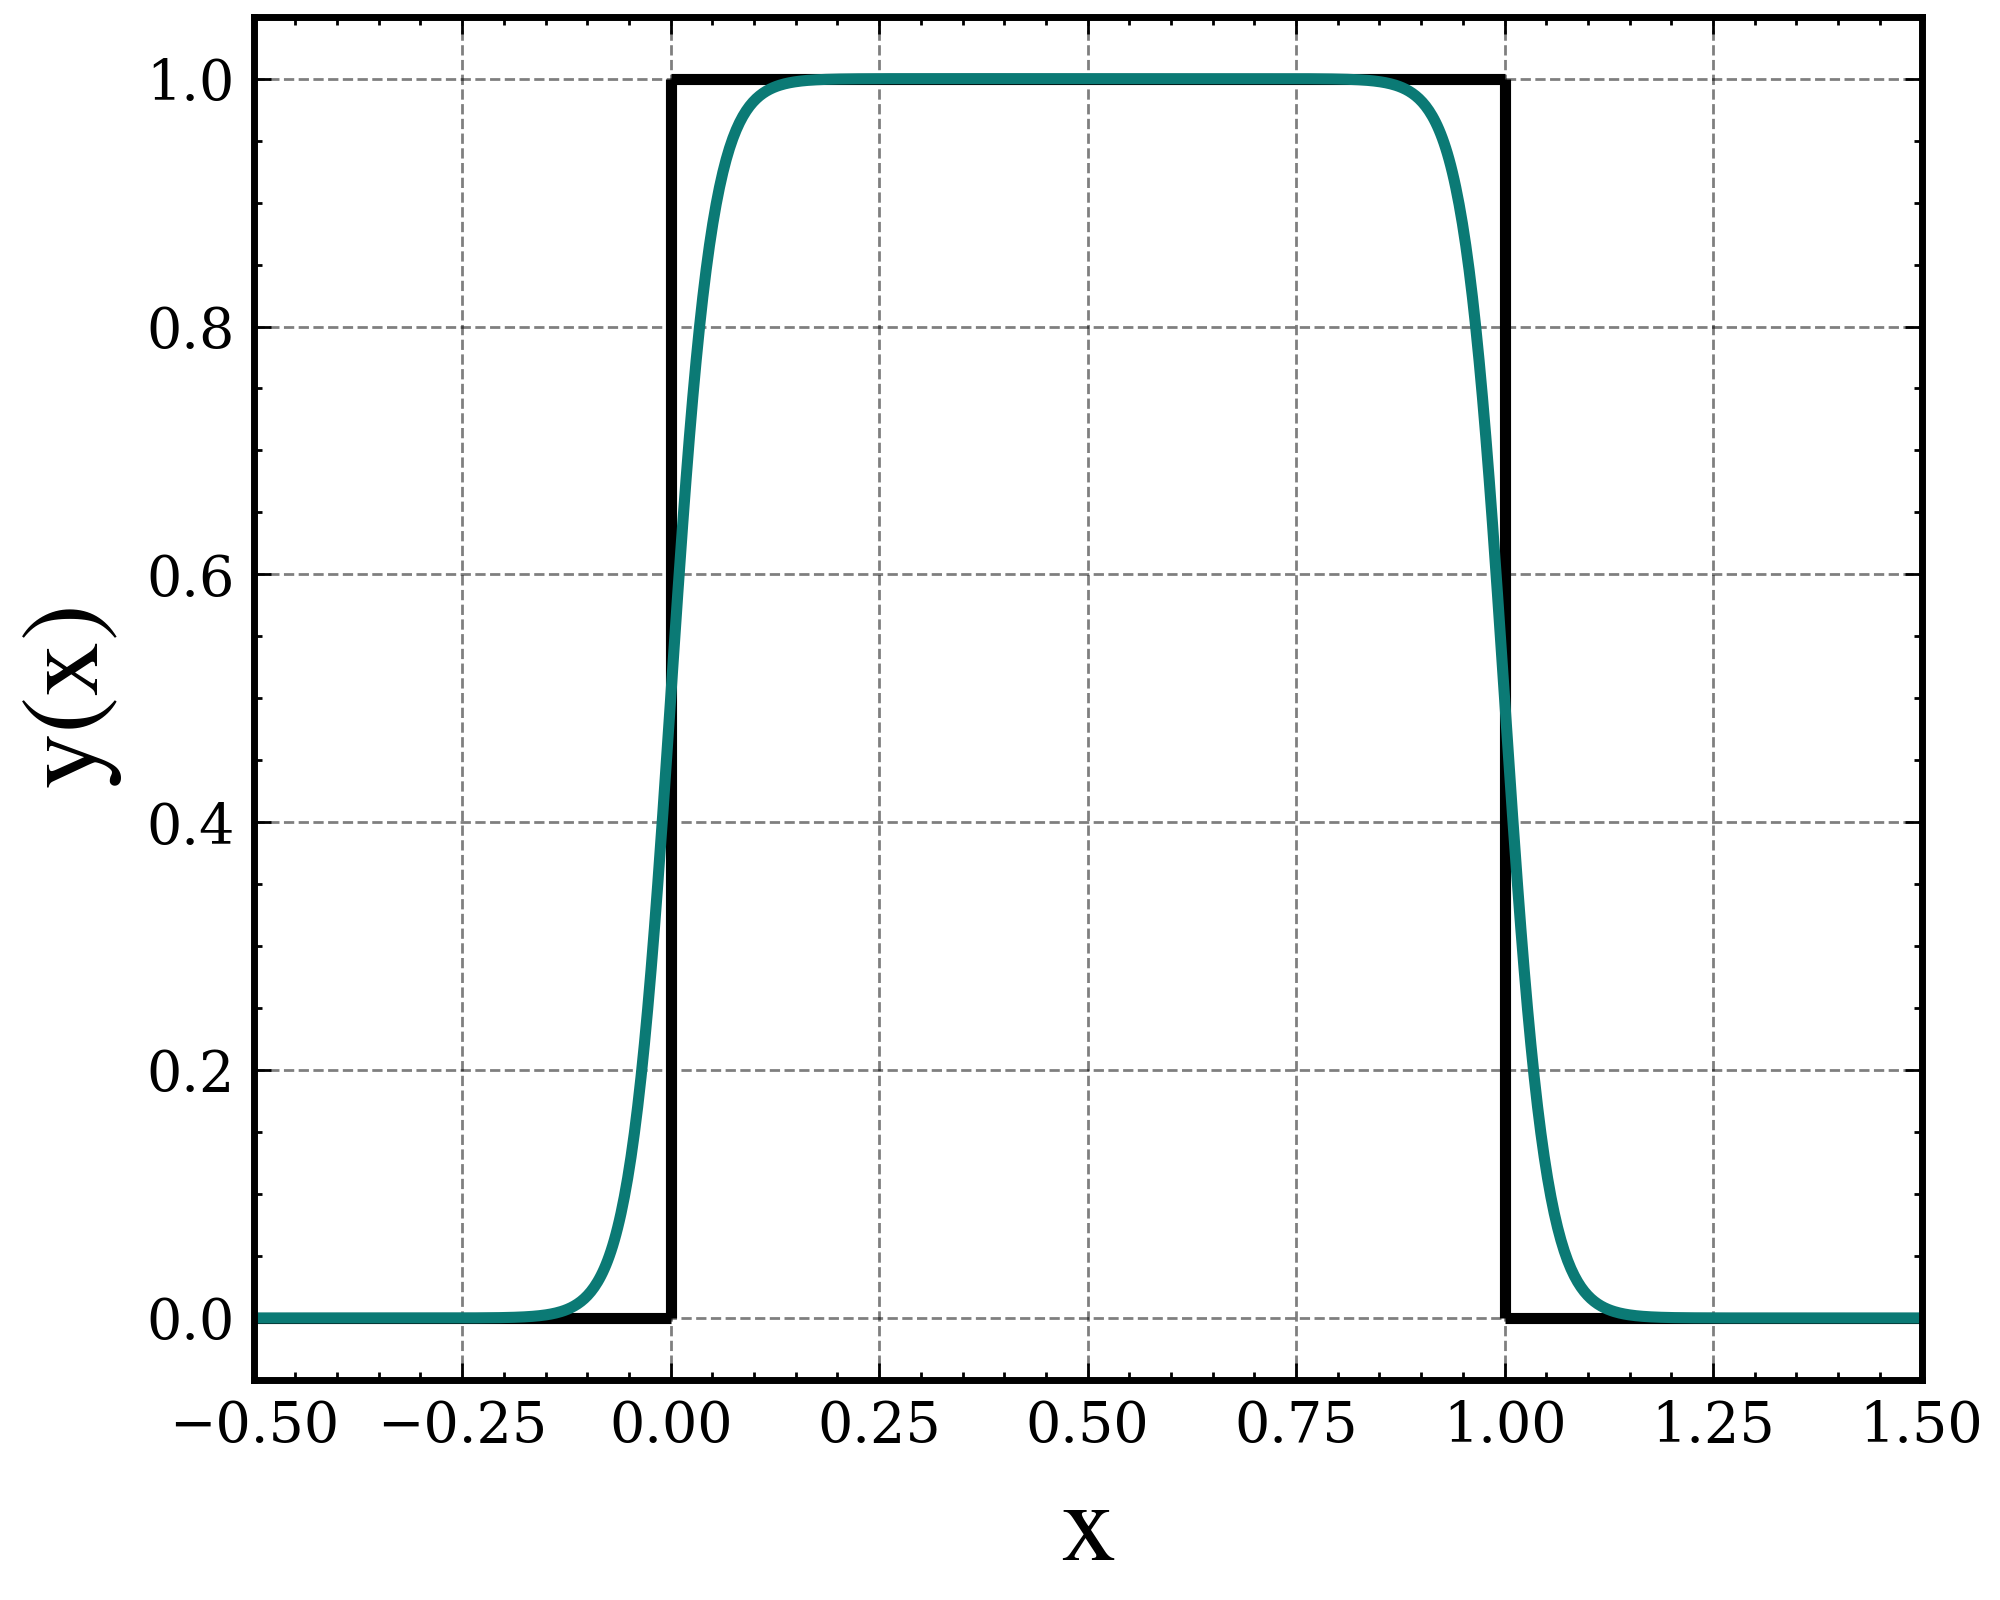
\includegraphics[width=1\textwidth]{img/ML/MLP_unit_impulse.png}
        \caption{Unit impulse (in black) and the output of the MLP shown in cyan approximating the impulse. }
        \label{fig:MLP_approx}
    \end{subfigure}
        \caption{A simple multilayer perceptron (MLP) with a single hidden layer and a $\tanh{}$ activation function is able to approximate a unit pulse function. From left to right and top to bottom, the three biases are $\{0, 20, 0\}$ and the four weights are $\{20, -20, 1/2, 1/2\}$.}
        \label{fig:ML MLP approx}
\end{figure}

This theoretical result can be easily visualized be understanding how a simple fully connected network (a multilayer perceptron, MLP) can approximate a unit impulse function. It is then enough to recall that a linear combinations of step functions can approximate any integrable function. In \cref{fig:MLP} we show a MLP consisting of an input neuron, and output neuron and a hidden layer with two neurons with a $\tanh{}$ activation function.
From left to right and top to bottom, we set the three biases as $\{0, 20, 0\}$ and the four weights as $\{20, -20, 1/2, 1/2\}$. The resulting MLP then produces the approximation shown in \cref{fig:MLP_approx} of the unit impulse over $[0,1]$. By expanding the number of neurons in the hidden layer we could approximate impulse functions of arbitrary width and height and centered at every arbitrary value. The high degree of expressivity of neural networks makes them particularly suited to parametrically approximate complex non-linear relationships between variables that would otherwise be intractable.

\begin{figure}
    \centering
    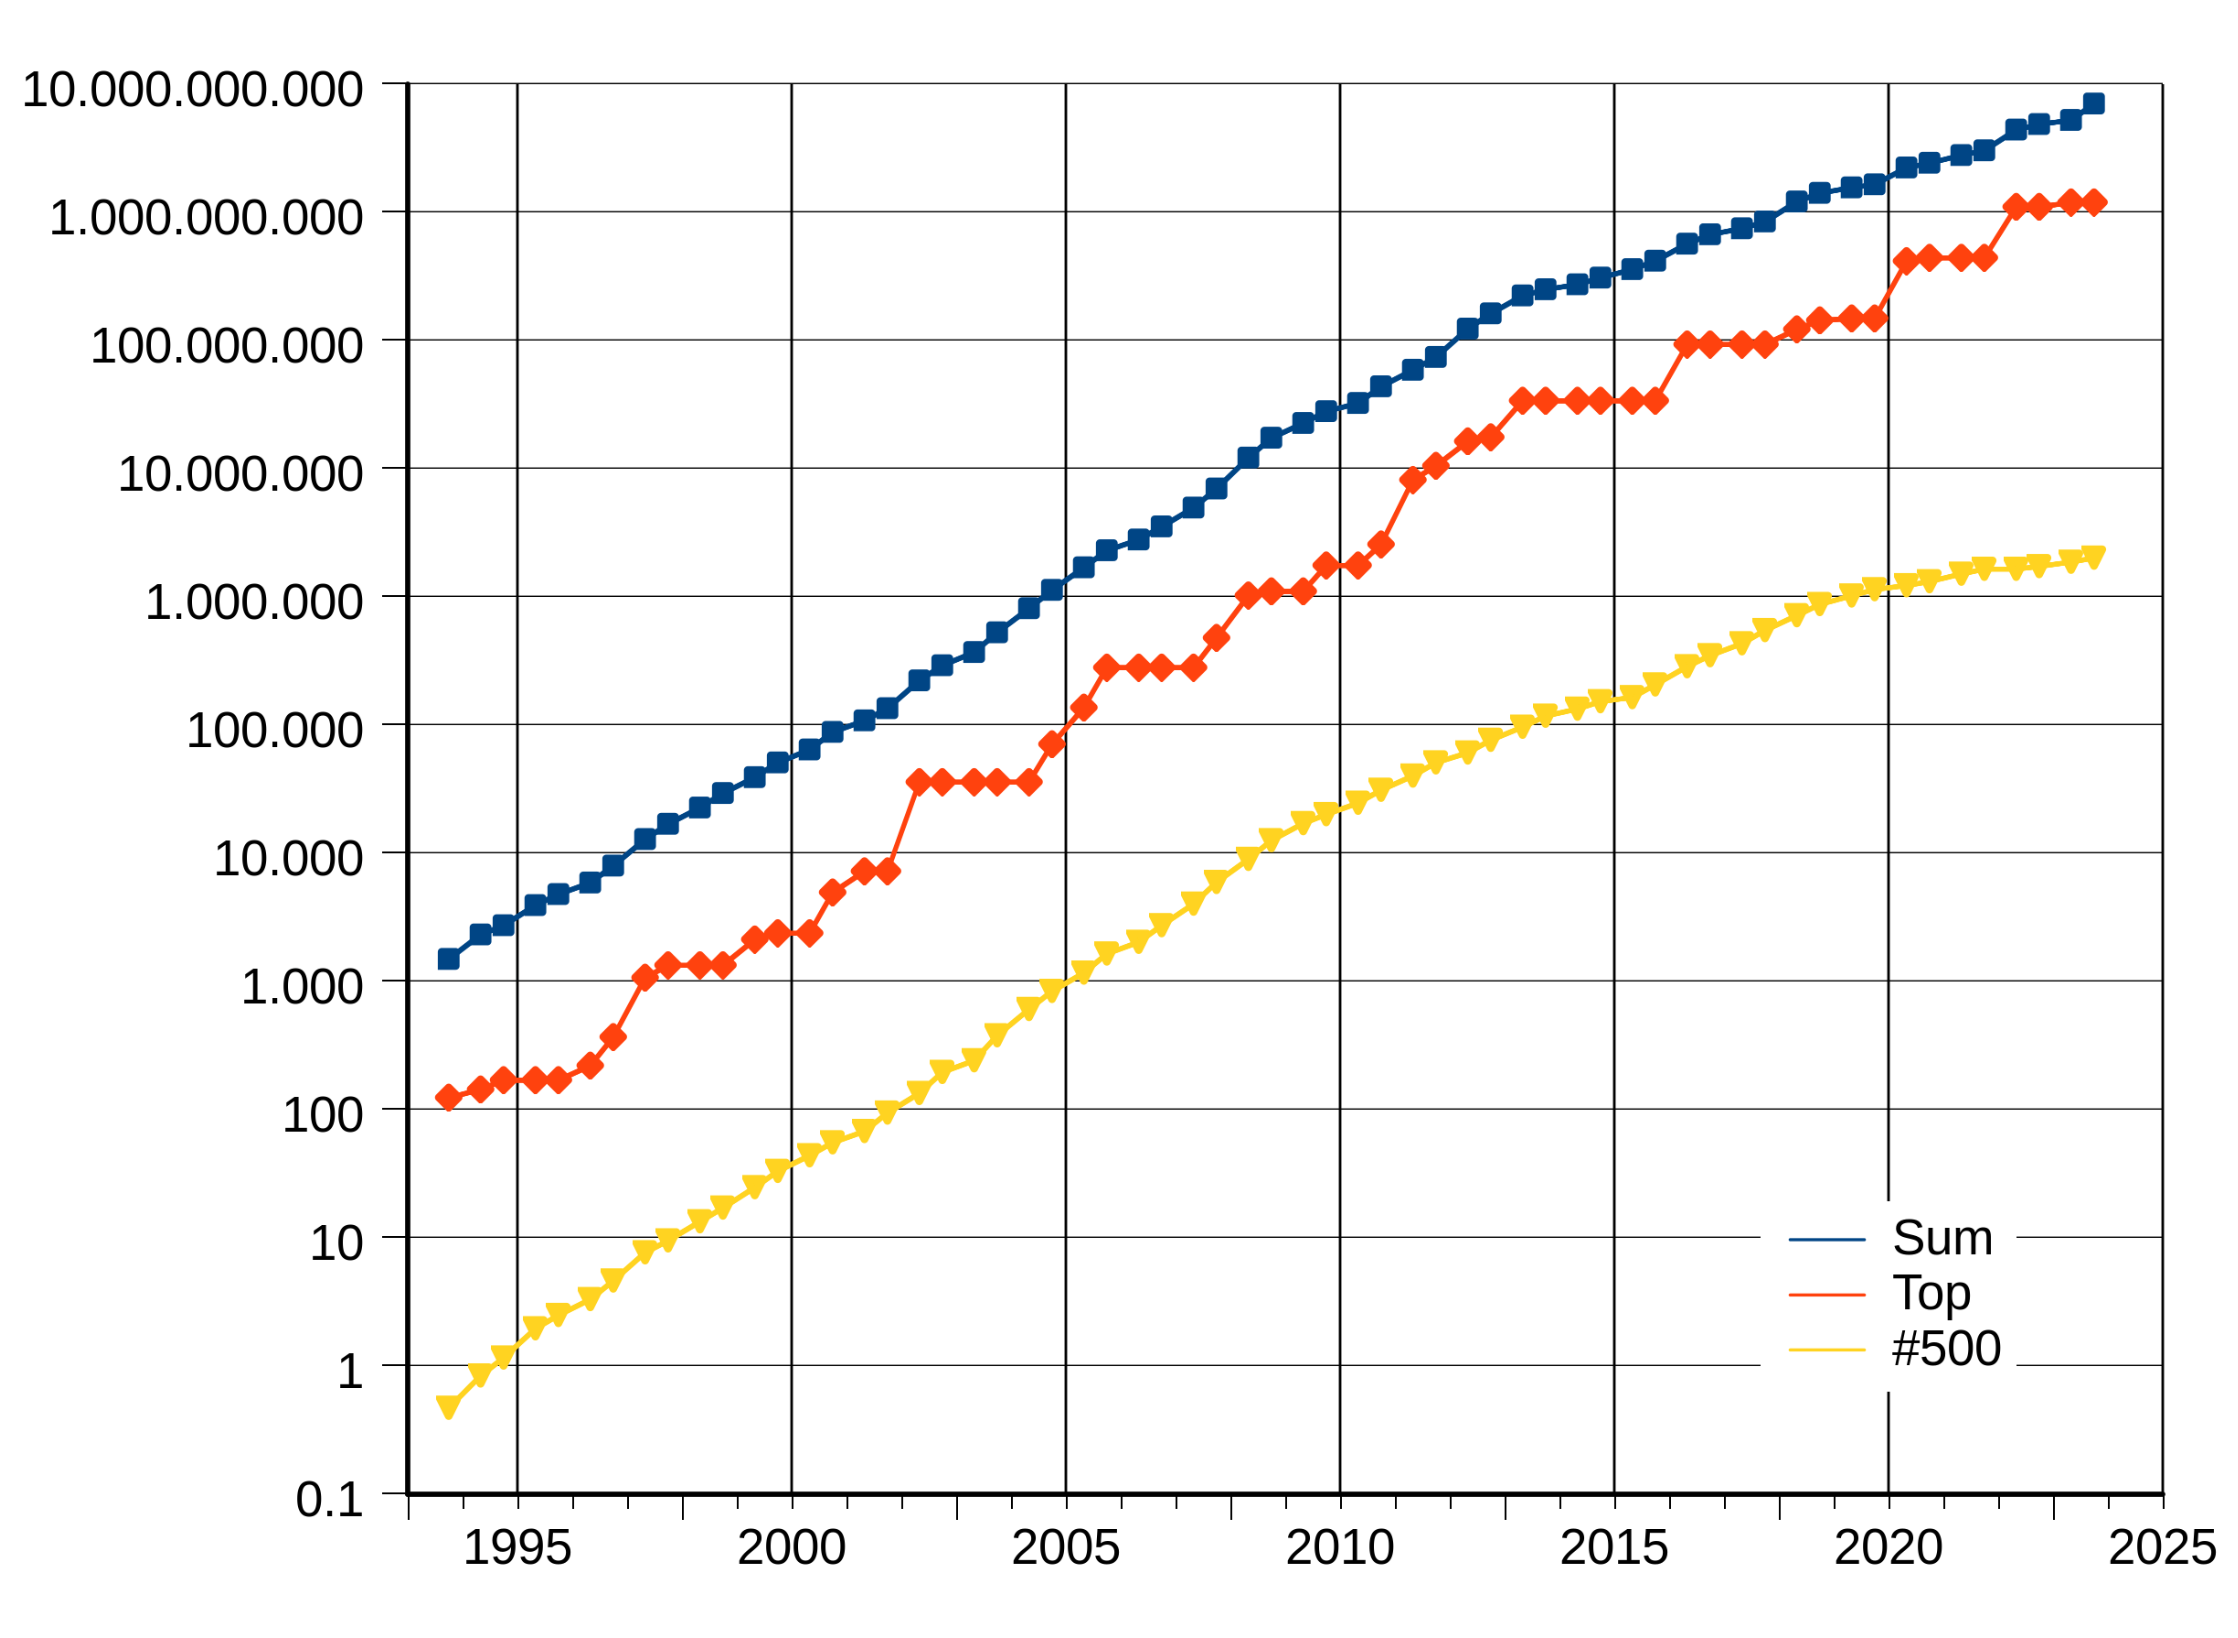
\includegraphics[width=0.7\linewidth]{img/ML/HPC.png}
    \caption{Evolution of the largest supercomputers in the \href{https://top500.org}{\textsc{TOP500}} list  in recent years (x-axis). The y-axis shows the peak performance in GFLOPS for the first-ranked computer (red), the last-ranked computer (yellow), and the cumulative power for the top-500 computers (blue). Source: \href{https://en.wikipedia.org/wiki/History_of_supercomputing}{Wikipedia}.}
    \label{fig:ML_HPC}
\end{figure}


Theorem \ref{th:aprox} establishes a theoretical aspect of neural networks supporting their utility, but it does not provide a method (nor does it guarantee the existence of any) to find networks that approximate a particular function of interest. The process of fitting a statistical model (such as a neural network) to a dataset of interest in know as \emph{supervised learning}, an constitutes one of the main aspect of this work, as we will explain in the rest if this section.
In recent years, the main points have allowed the rapid expansion of machine learning, marking a new era in the use of large parametric networks for real-world problems:

\begin{itemize}
    \item \textbf{Hardware development.} The rapid (quasi-exponential)growth in computer power in recent years, as exemplified by Moore's law \cite{Moor_law} means that extremely deep and complex models can now be trained and effectively used. As a reference, the language models \textsc{LLAMA} by Meta can have over 65 billion parameters \cite{Llama}. To handle this amount of data, High Performance Computing (HPC) infrastructures (such as supercomputers) are needed. Figure \ref{fig:ML_HPC} shows the rapid evolution for the top supercomputers in the world, as ranked by the TOP500 list\footnote{\url{https://top500.org}}. In 1993, the \textsc{Fujitsu Numerical Wind Tunnel} in Japan topped the list with 124 GFLOPS. In 2023, the list is topped by \textsc{Frontier} in the United States, with over 1000 PFLOPS, which corresponds to an 8000-fold improvement. Progress in hardware technology as also been remarkable. For instance, Graphics Processing Unit (GPU) are now common when training machine learning models. As a last example, in May 2017, Google introduced an architecture known as Tensor Processing Unit (TPU) especially designed to accelerate neural network operations \cite{TPU}. HPC also enables the generation of synthetic datasets from simulations, that can then be used as training datasets. We will leverage this idea in the rest of this work.


    \item \textbf{Computationally-efficient algorithms.} Together with hardware development, we have seen a rapid evolution of computational and mathematical algorithms in the field of statistical learning that have enabled the efficient utilization of HPC resources. The epitome of such algorithm might be \emph{backpropagation} \cite{backprop} which is the most common algorithm used in the training phase to update the weights when deploying a neural network. Together with backpropagation, a growing set of optimizers for deep learning problems have been developed. A popular choice is \textsc{Adam}, which was originally published in 2017 \cite{adam}.

    \item \textbf{Availability of large datasets.} The advent of next-generation instruments and data-collections systems provides the scientific community with increasingly large datasets. Prominent examples in the field of astronomy include Gaia \cite{gaia}, whose third data release (DR3) includes 10TB of data for 1.46 billion sources\footnote{\url{https://www.cosmos.esa.int/web/gaia/dr3}}, or the Euclid telescope, expected to deliver 850 GB of compressed data per day\footnote{\url{https://sci.esa.int/web/euclid/-/46661-mission-operations}}. At last, in \cref{fig:Supernovas_per_year} we show the evolution in the number of SNe discoveries per year. The figure as been obtained from \cite{SN_year}.



    
\end{itemize}

\begin{figure}
    \centering
    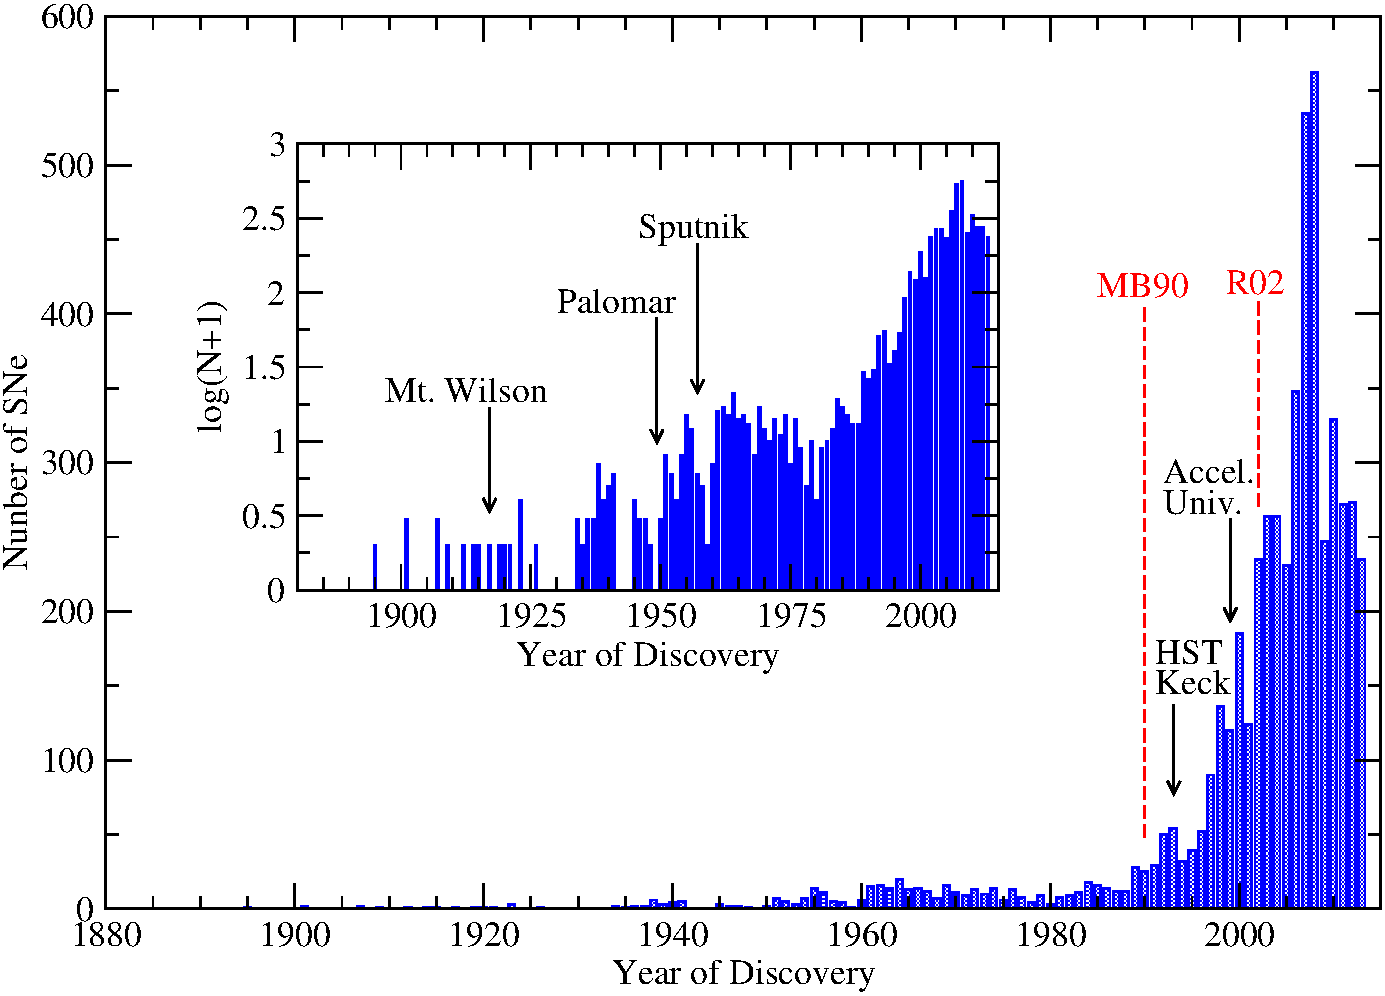
\includegraphics[width=0.7\linewidth]{img//ML/fig1_color.pdf}
    \caption{Histogram showing the number of SNe discovered each year as given by the Asiago Supernova Catalogue.}
    \label{fig:Supernovas_per_year}
\end{figure}



Let us demonstrate the relevance, pertinence, and range of applicability of machine learning methods in astronomy and cosmology by examining recent endeavours documented in the literature. While not exhaustive, this examination provides a broad overview of previous efforts in the field, and illustrates some recent successes of machine learning-oriented approaches in data-driven problems.
\par
The abundance of data from surveys covering large regions of the sky aimed at targeting QSOs makes supervised statistical techniques a particularly attractive data analysis technique. For reference, the main quasar sample in the data release number 16 for the Extended Baryon Oscillation Spectroscopic Survey (eBOSS) contains 434820 targets with redshifts in the range $0.8<z<2.2$ \cite{eboss}. The prediction of the intrinsic Lyman-$\alpha$ emission line from high redshift QSOs is a non-trivial problem that has important implication in the study of IGM damping wings and the reionization of the later \cite{MiraldaEscude_IGM}. Reconstruction techniques often rely on the correlation of the Lyman-$\alpha$ peak with other observable lines and information redward of the Lyman-$\alpha$ line. Machine learning approaches are then suitable to connect the unattenuated information redward of the Lyman-$\alpha$ peak with its intrinsic profile. In \citetitle{qso_challenge} \cite{qso_challenge}, the authors perform an in-depth comparison of different state-of-the-art techniques based on statistical learning. The authors blindly evaluate their performance on two QSOs samples randomly extracted from X-Shooter and BOSS with $3.5<z<4.5$, in such a way that selecting samples already used in the training data-set was avoided. The various techniques range from principal component analysis (PCA) approaches, such as \cite{Bosman2021_pca}, to deep learning networks \cite{Liu2021}. The authors conclude that the better performing pipelines consistently rely on machine learning approaches. The authors caution against overreliance on machine learning techniques due to their potential lack of statistical uncertainty, which is one of the main aspect that we will develop in this work.


\par
Parameter inference on WDM using deep learning has already been tentatively explored in the recent literature.
The paper \citetitle{wdm_from_field} \cite{wdm_from_field}, which is especially relevant for this work, demonstrates that neural networks can be used to recovered WDM parameters from observed field density images. The authors present a suite of 1500 cosmological N-body simulations with varied WDM mass in the range 2.5 to 30 KeV. Field density images of size 25h$^{-1}$Mpc, with varied image resolution, simulation resolution and redshift (in the range $0\leq z \leq 5$) are extracted from the simulation runs. The images are augmented usual standard techniques (such as image rotation) and then incorporated into training datasets. The authors use a Convolutional Neural Network (CNN) trained to directly predict WDM masses based on an input density field image. Their fiducial convolutional network trained with the set of highest resolution image is able to accurately recover WDM masses with an accuracy of $\pm$1 KeV for models up to 10 KeV. After this threshold value, the network is no longer able to recover the true mass as predicts an approximately constant mass, see \cref{fig:ML paper wdm field}. Note that in the architecture presented by the authors, the network is also trained to predict an uncertainty estimate. Another interesting insight offered by this paper refers by the capacity of neural network to make use of the full information contained on a field distribution (in this case, the density field). By training a network on a full density field image the models learns the relevant properties of the field that can lead to an accurate parameter prediction. The authors train another model only on summary statistic, in particular, on the density power spectrum, and compare its performance with their fiducial model trained on the full images. The model trained only on the power spectra shows a significantly degraded performance, with higher uncertainties and accurate prediction only up to 5.5 KeV. This illustrate how deep learning techniques can help harvesting the full information present in a field (or generally, in a complex input tensor).


\begin{figure}
    \centering
    \begin{subfigure}[b]{0.53\textwidth}
        \centering
            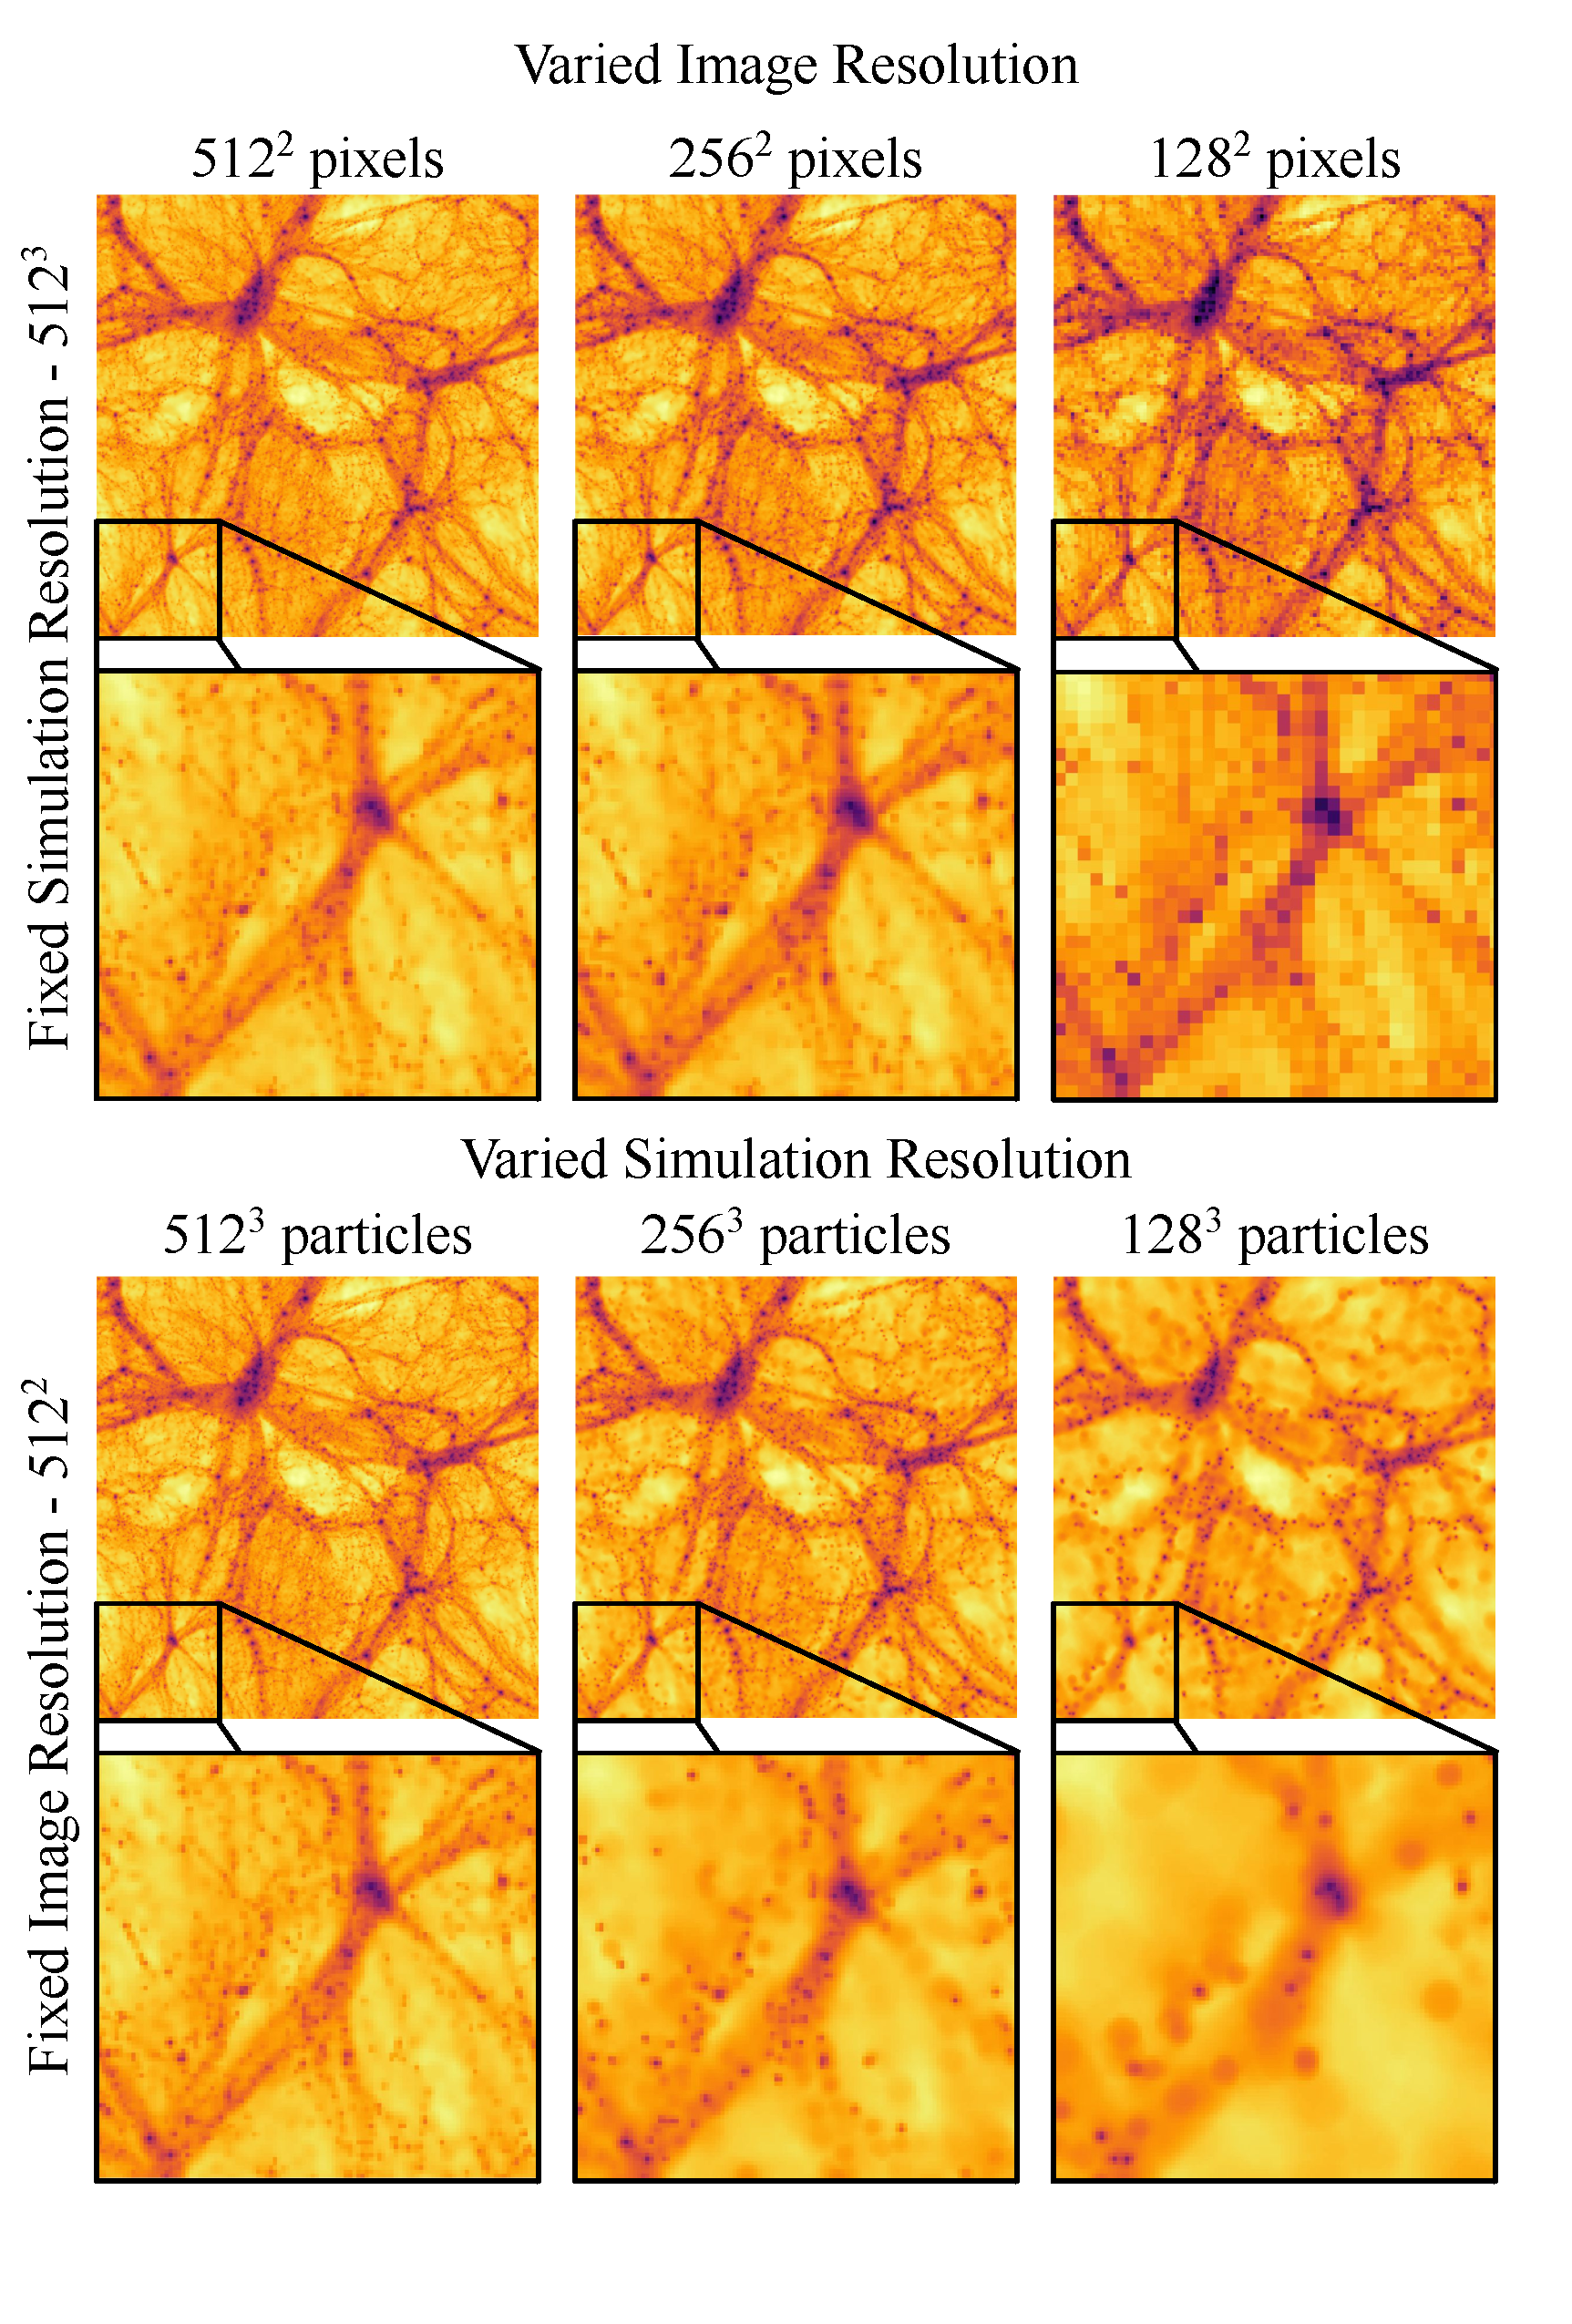
\includegraphics[width=1\textwidth, trim={0 22.2cm 0 0},clip]{img/ML/CAMELS_Images_Update.pdf}
    
    \end{subfigure}
    \hfill
    \begin{subfigure}[b]{0.45\textwidth}
        \centering
        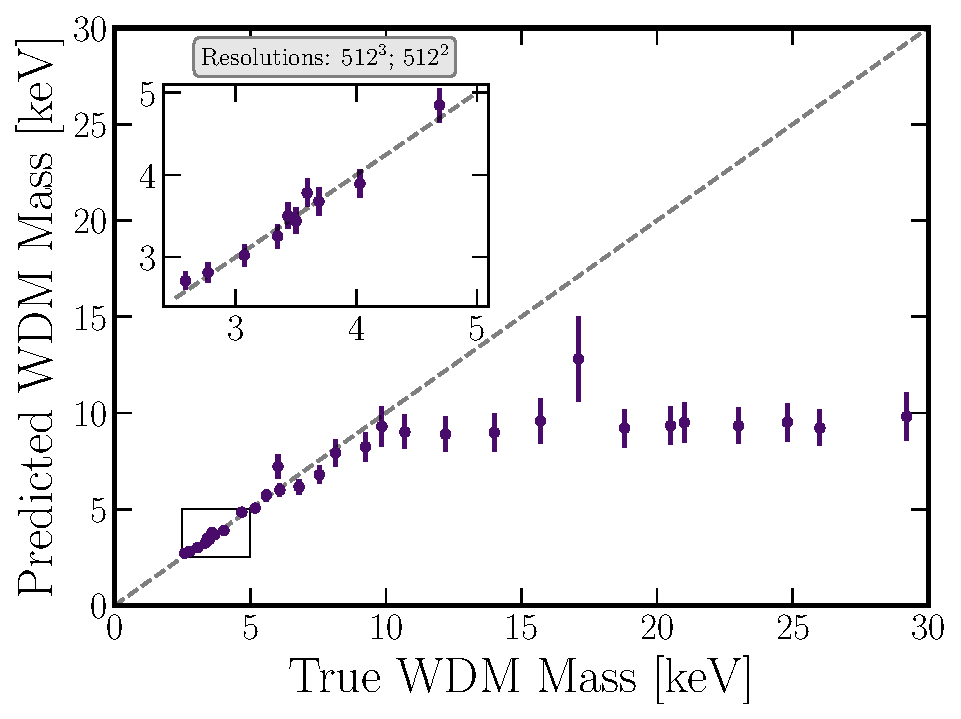
\includegraphics[width=1\textwidth]{img/ML/results_fixed_sim512_res512_z0.pdf}     
    \end{subfigure}
        \caption{Figure extracted from \cite{wdm_from_field}. The left panel shows a sample image density field used in the training data by the authors, with varied image resolution. The right panel shows a sample a predicted WDM masses versus the true WDM mass of the simulation for their fiducial neural network, which can accurately recover the WDM model within a 1 KeV accuracy up to 10 KeV.}
        \label{fig:ML paper wdm field}
\end{figure}

Another recent use of deep learning to analyse IGM data can be found in the paper \citetitle{lynna} \cite{lynna}, where authors harvest the field level potential of residual convolutional networks to perform inference on the thermal parameters of the IGM, namely $T_0$, the temperature at mean density, and $\gamma$, the slope of the temperature-density relation. Their model is trained on simulation boxes with side-length 120 Mpc from which $10^5$ sightlines are extracted and processed to produce mock Lyman-$\alpha$ spectra. The simulation boxes are run with different thermal parameters, by sampling 121 $(T_0,\gamma)$ combinations in the parameter space. The network is trained on 24000 labeled spectra from the mix of thermal models, and the architecture is designed to predict a mean value for the thermal parameters as well as an estimate for the parameter covariance matrix. Figure \ref{fig:ML LYNNA} shows the scatter in the point predictions for $(T_0,\gamma)$ for a set of 4000 unseen test spectra. The true parameter values, shown as dashed lines, are recovered by the average of the point predictions, shown as the dark green cross. The authors also perform a comparison with an inference pipeline based on the traditional transmitted flux power spectrum, and find that the posterior constraint using the machine learning field-level approach are 5.65 times tighter.


\begin{figure}
    \centering
    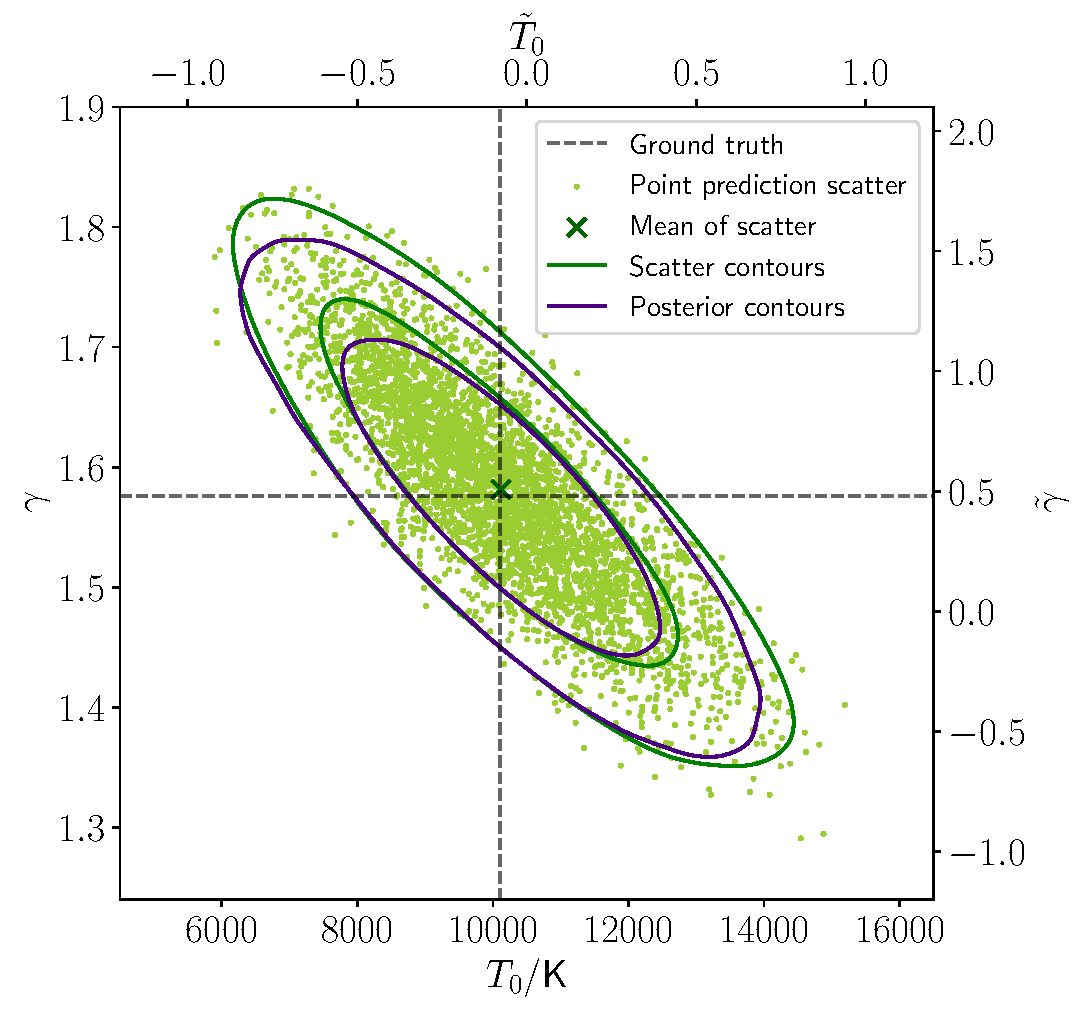
\includegraphics[width=0.6\linewidth]{img//ML/scatter__and__posterior_contours_fiducial_tdr.pdf}
    \caption{Figure extract from \cite{lynna} showing the performance of the neural network recovering thermal parameters on a set of unseen skewers. The true parameter values, shown as dashed lines, are recovered by the average of the point predictions, shown as the dark green cross.}
    \label{fig:ML LYNNA}
\end{figure}






\section{Fundamentals of (Bayesian) Neural Networks}

A very general regression problem in statistical learning \cite{James2021} arises when we observe a quantity $Y$ that is assumed to depend on an independent variable $X$ through a relation of the form

\begin{equation}
    Y = f(X)+\mathcal{N}(0,\sigma),
\end{equation}
where $f$ is a function defining the relation $Y=Y(X)$ and $\mathcal{N}(0,\sigma)$ is an error term modeling a zero-mean Gaussian noise. The problem then consists of estimating $f$ given a sample of observations $\{ X_i, Y_i\}_i$ to obtain a functional form $\hat{f}$ that can then be evaluated to obtain predictions. Following the examples in section $\ref{sec:motiv_ml}$, $X$ might be the flux spectra redward of the Lyman$-\alpha$ peak, and $Y$ might then be the intrinsic shape of the Lyman$-\alpha$ peak in the quasar spectra. The noise then is produced by different sources, for instance, associated with the instrumental devices. We could then use the obtained $\hat{f}$ to predict to intrinsic Lyman$-\alpha$ peak of a QSO, $\hat{f}(X)$, when we only have information about the spectrum redward of it, $X$. As it is expected, the quality of our prediction depends on how accurate is the approximation $\hat{f}$ with respect to $f$, but also on how noisy our data is. In fact, we see that, if the true quantity associated with $X$ is $Y$:

$$(Y-\hat{f}(X))^2=(f(x)+\mathcal{N}(0,\sigma)-\hat{f}(X))^2.$$
Taking expected values and noting that the only stochastic component here is the noise, we obtain 
\begin{equation}\label{eq:var_noise_model}
    \mathbb{E}[(Y-\hat{f}(X))^2]=(f(X)-\hat{f}(X))^2+\sigma^2.
\end{equation}
In \cref{eq:var_noise_model}, the first term of the right-hand side represents the error produced by approximating $f$ by $\hat{f}$, while the second term is a theoretical limit imposed by the noise properties.

Parametric methods represent a powerful statistical learning tool to approximate the target relation $f$ between variables.
Methods such as linear regression, which approximates $Y=f(X)$ using a linear functional form on the parameter values, offer limited flexibility in terms of approximating complex relations but allow for a high degree of interpretability of the model. On the other end of the spectrum, deep learning models offer a large degree of expressivity (see \ref{sec:motiv_ml}), but interpretation of individual parameters is often not possible. Increasing the number of parameters can also cause the model to learn from spurious structures in the finite data sample, or the learn from possible noise correlation. This process, known as \emph{over-fitting}, can significantly impact the predictive performance of the model when predicting on unseen data. Multiple techniques have been explored to mitigate over-fitting \cite{overfitting}, we will adopt some of them in this work and explain them in the following sections.

In this section we will discuss the basic workflow involving a deep learning model in a general and abstract scenario. We will restrict ourselves to the topics that are relevant for this work, and later explain in detail how we implement this workflow for our problem.
The general workflow when working with a deep learning statistical model under supervised learning includes the following phases:
\begin{enumerate}
    \item Collecting/data and processing it to generate a training dataset. This requires specific domain expertise to assess the quality and representability of the data.
    \item Designing a deep learning architecture, i.e., a computational graph that depends on a set of parameters and that generates target outputs from the input data.
    \item Using the available data to train the model. This is done by optimizing the model parameters by minimizing a selected loss function.
    \item Assessing the performance of the network a validation dataset, previously unseen.
    \item Using the model on real unseen data to make predictions.
\end{enumerate}

\subsection{Dataset generation, data augmentation and overfitting.}\label{sec: dataset}

In a general real-world setting only a finite dataset is available to us, for instance, obtained from observational procedures.
That is, we have a set of pairs $\mathcal{D}=\{X_i,Y_i \}_{i=1}^{i=N}$ of $N$ observations from an input-output pairs, distributed according to some distribution $F(X,Y)$:
\begin{equation}
    (X_i,Y_i) \sim F, i=1,...,N.
\end{equation}
Of course in general, we don't have access to the distribution of this population (i.e., the function $f$ describing the data relation $Y=f(X)$), otherwise we would already have a perfectly accurate model, and we would not to invoke any statistical learning tool.
The challenge is then to use our sample $\mathcal{D}$ to infer properties of the population.
Since we don't have access to the generating function $f$, we cannot assess the general performance of the model on arbitrary input data.
For this purpose, the training dataset $\mathcal{D}$ is typically split into two disjoint subsets $\mathcal{D}=\mathcal{D}_T \sqcup \mathcal{D}_V$, where $\mathcal{D}_T$ represents the subset of the data used for training, and $\mathcal{D}_V$ represents the subset of the data used to validate the model and assess its performance.
The central idea behind this split is to be able to validate the model on data that has not been used in the training process, allowing for an estimation of the model's generalization to the population given by:
\begin{equation}\label{eq_ch3:global_loss}
    \varepsilon =\mathbb{E}_F[\mathcal{L}(Y,\hat{f}(X|\mathcal{D}_T))],
\end{equation}
where $\mathcal{L}$ is a loss function.
The exact form in which the $\mathcal{D}$ is split needs chosen a priori, with the aim of having a representative sample of the population.
A common easy-to-implement strategy is to randomly select the samples in $\mathcal{D}$ that will be part of $\mathcal{D}_V$ and distributing them according to a ratio, that is commonly taken to in the range $60-80\%$, meaning that a larger percentage of $\mathcal{D}$ is dedicated to training.
In this case, an unbiased estimator of $\varepsilon$ is
\begin{equation}
    \hat{\varepsilon}=\frac{1}{|\mathcal{D}_V|}\sum_{i=1}^{|\mathcal{D}_V|}\mathcal{L}(Y_i,\hat{f}(X_i)),
\end{equation}
where the sum runs over the validation dataset.
More complex strategies that take into account the topology of the data exist and allow for an optimal training-valiation split \cite{data_split}. 
The validation subset can also be sequentially cycled through all the available samples in a series of methods called \emph{cross-validation} \cite{cross_validation}. Cross-validation uses all available data in a validation stage by retraining a model on different disjoint splits of the data. This allows for a more precise evaluation of the model.

If the training subset $\mathcal{D}_T$ is not representative of the population, then the global error in \cref{eq_ch3:global_loss} will be large, and the model will not be able to learn the general properties of the data.
This can cause the model to overfit and learn from spurious correlation in the data and noise, and can be encouraged by having an excessive number of free parameters.
Overfitting is not an intrinsic characteristic of deep-learning models, can can also be seen for instance in simple polynomial regression when the number of ``independent'' points exceeds the order of the fitting polynomial.
Figure \ref{fig:ML overfit poly} illustrates the simple example of polynomial regression overfitting the training dataset as the order of the polynomial increases. Note how, by construction, the fit becomes increasingly accurate on the training data, but looses generalization power on unseen points.
\begin{figure}
    \centering
    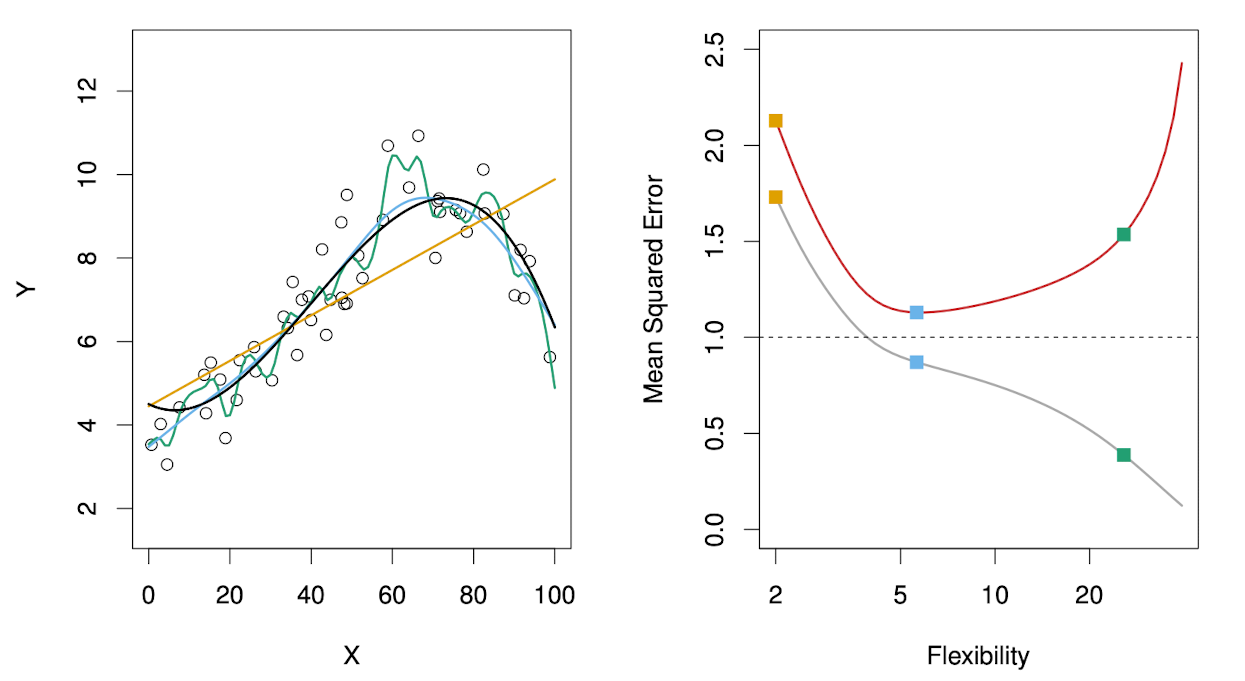
\includegraphics[width=0.7\linewidth]{img/ML/poly_overfit.png}
    \caption{The left panel shows the data points (with added noise) generated from a function $f$ in black. Three generative polynomial models are fitted to the data: linear regression in orange, and two smoothing splines in red and blue. The right panel shows the fitting error as a function of the polynomial degree, i.e., the flexibility of the model. The gray curve shows the error on the training dataset, which is monotonically decreasing. The red curve shows the error on the validation dataset, which initially decreases but then grows as the model overfits the training data. Figure extracted from \cite{James2021}. }
    \label{fig:ML overfit poly}
\end{figure}

The training data $\mathcal{D}_T$ can be artificially extended using \emph{data augmentation} techniques \cite{data_augmentation} to generate new training points from existing points. Data augmentation aims at presenting the model with data that maintains intrinsic properties of the original data but varies other features that should not affect the prediction. This approach can be understood to be inspired by symmetry considerations\footnote{A strawberry is a strawberry regardless of its orientation} and is particularly useful in computer vision tasks. Some common data augmentation techniques for image processing include:

\begin{itemize}
    \item Basic geometric transformations such as rotation, translation or flipping an image (or field) are efficiently implemented. Cropping can also be easily implemented, but changes the dimensionality of the data.
    \item Basic color space manipulation in colored images, including isolating a single color channel, or modifying the brightness of an image.
    \item Noise injection during training is particularly useful in making neural networks robust against noisy and corrupted data. Note that this can be relevant if the data we are expecting to use the trained model on has noisy (for example instrumental data from a spectrograph). The noise can be randomly drawn from independent distributions, or drawn from a noise model if we have additional insights on how to model it.
    \item Convolutional operations with kernels, such as the Gaussian kernel to apply a limited spatial resolution (blurring), or the Sobel kernel for related to edge detection.
\end{itemize}


\subsection{Deep learning architecture}\label{sec:deep learning archi}
The network architecture defines the parametrization of the function that approximates the true underlying relation between input and output data points. In this section we briefly explore some basic building blocks used when constructing a deep learning network.
A neural network (NN) $\phi$ is a computational graph with an input tensor $X$ and an output tensor $Y$ and parametrized by a set of values $\omega$ that define a functional model
\begin{equation}
    Y=\phi(X|\omega)\equiv \phi_\omega (X).
\end{equation}
For simple linear topologies a NN can be specified given a set of connected \emph{layers} that carry out the elementary operations. These layers can be grouped in \emph{blocks} to form subnetworks inside a NN. Three of the simplest layer architectures are \emph{feedforward} layers (also known as \emph{dense} layers), convolutional layers, and residual layers. Since they will be of use in our machine learning workflow, we will discuss their exact structure.

\begin{itemize}
    \item In the simplest feedforward network, such as the one illustrated in \cref{fig:MLP}, all layers are linearly connected with an additional activation function, leading to a model of the form

    \begin{equation}
        \begin{aligned}
            &X=\boldsymbol{l}_{0}, \\
            &\boldsymbol{l}_{i}=s_{i}(\boldsymbol{W}_{i}\boldsymbol{l}_{i-1}+\boldsymbol{b}_{i})\quad\forall i\in[1,N], \\
            &Y=\boldsymbol{l}_{N},
        \end{aligned}
    \end{equation}
    where $l_i$ are the layers, $W_i$ the weights, $b_i$ the biases, $\sigma_i$ the activation functions and $N$ the number of layers.
    
    
    \item Convolutional layers are especially useful in signal processing and computer vision problem. They incorporate multiple convolution operations on the input array. The parameters of the layers define the exact way the convolution is performed. Consider for illustration purposes the case of an input 2D array of size $(N,N)$. The convolutional layer is internally parametrized by a kernel $\omega$ of shape $(m,m)$ such that the input $X$ to the layer is transformed as
    \begin{equation}
        Y_{i,j}=\sum_{a=0}^{m-1} \sum_{b=0}^{m-1} \omega_{ab} X_{i+a,j+b}.
    \end{equation}
    The output size will be $(N-m+1,N-m+1)$. Lastly, a user-specified non-linearity is applied. The implementation of convolutional layers in machine learning APIs is usually done by specifying a kernel size and a set of auxiliary parameters. For instance, a single layer can have multiple independent kernels, can apply padding to the input array before convolving, etc.

    \item Residual layers implement a skipping connection within another layer, typically a convolutional one. A skipping connection adds the input tensor to the output tensor:
    \begin{equation}
        Y=T(X)+X,
    \end{equation}
    where $T$ is other neural layer. A relevant property, both from the theoretical and practical viewpoints, is that the derivative of the output tensor $Y$ with respect $X$ to X always include an identity term that tends to prevent it from being zero. This allows the information to flow easily in deep architectures, speeding up training and limiting overfitting \cite{residual_paper}.
    \item Batch-normalization layers \cite{ioffe2015batch} address the training difficulty encountered when the input tensors vary significantly from a sample to another. These differences cause different network weights to be adjusted simultaneously in opposite directions, which ultimately impairs training. Batch-normalization layers simply aim at normalization each tensor input feature when we feed a batch of samples to a network. A batch-normalization layer as 2 internal parameters $\gamma,\beta$ for each input features, that are applied as a linear transformation after normalization. If we consider an input feature $x$ (that is, a component of $X$), and a bath of samples $\{x_1,...,x_m \}$, then a batch-normalization layer is implemented as:
    \begin{equation}
        \begin{aligned}
            \mu& =\frac1m\sum_{i=1}^mx_i  \\
            \sigma^2& =\frac1m\sum_{i=1}^m(x_i-\mu)^2  \\
            \widehat{x}_i& =\frac{x_i-\mu}{\sqrt{\sigma^2}}  \\
            \mathbf{BN}_{\gamma,\beta}(x_i)&\equiv \gamma\widehat{x}_i+\beta
            \end{aligned}
    \end{equation}
    


    \item Max pooling layers are usually added after convolutional layers to downsample, add translational invariance and hence make to network more robust against the presence of features in different spatial positions. Similar to a convolution, max pooling is done by sliding a kernel windows onto the input array, but now we select the maximum value within the window.
\end{itemize}
\begin{figure}
    \centering
    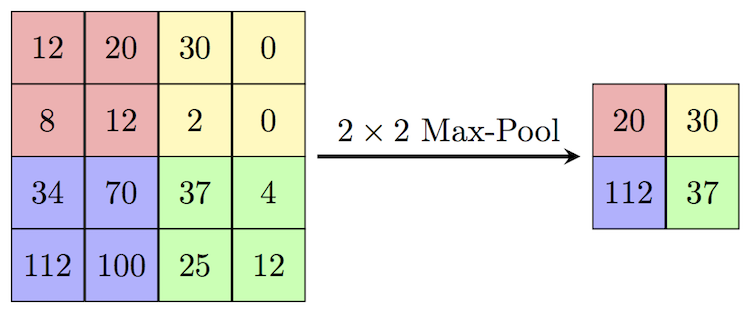
\includegraphics[width=0.6\linewidth]{img/ML/MaxpoolSample2.png}
    \caption{Max pooling operation with kernel size $(2,2)$}
    \label{fig:ML max pool}
\end{figure}

\subsection{Prediction uncertainty and Bayesian models}
In classical supervised deep learning, a neural network with weights $\theta$ is trained on some dataset $\mathcal{D}$ to produce a minimal cost estimator $\hat{\theta}$ for a predefined loss function. From the statistical point of view, this is a point estimate for each one of the network parameter. Point-estimate networks might lack explainability and generalize in overconfident ways to unseen data, and there is no obvious mechanism for such models to express their ignorance in such cases.


This is an analogous situation to classical parameter inference in statistic. From this perspective, the \emph{frequentist} approach to parameter estimation can be compared to point-estimate networks.
However, \emph{Bayesian} statistics \cite{bayesian_stat} has flourished in the last decades and is becoming the dominant statistical framework for data analysis inference problems. In the Bayesian paradigm, parameters are treated as random variables to reflect our ignorance about their ``true'' values. Our prior beliefs about the parameters $\theta$ are then updated in the presence of new data $\mathcal{D}$ using Bayes' theorem:
\begin{equation}\label{eq:Bayes theorem}
    P(H|D) \propto P(D|H)P(H),
\end{equation}
where $H$ is a certain hypothesis about $\theta$, $P(D|H)$ is known as the \emph{likelihood} and encodes the relation between the data generation and the parameters, and $P(H)$ reflect our prior beliefs. Bayesian frameworks have two main advantages. Firstly, they allow us to make our assumptions explicit by setting up the prior $P(H)$. This allows us to clarify, discuss and criticize prior knowledge in a clear way. Secondly, they provide a natural approach to quantify uncertainties in the inference parameters.


Bayesian neural networks are models that incorporate stochastic elements and that are trained using Bayesian inference techniques \cite{BNN_review}. This is generally implemented either by considering stochastic weights in the network, or by considering 
stochastic activations, see \cref{fig:ML BNN ilus}.

\begin{figure}
    \centering
    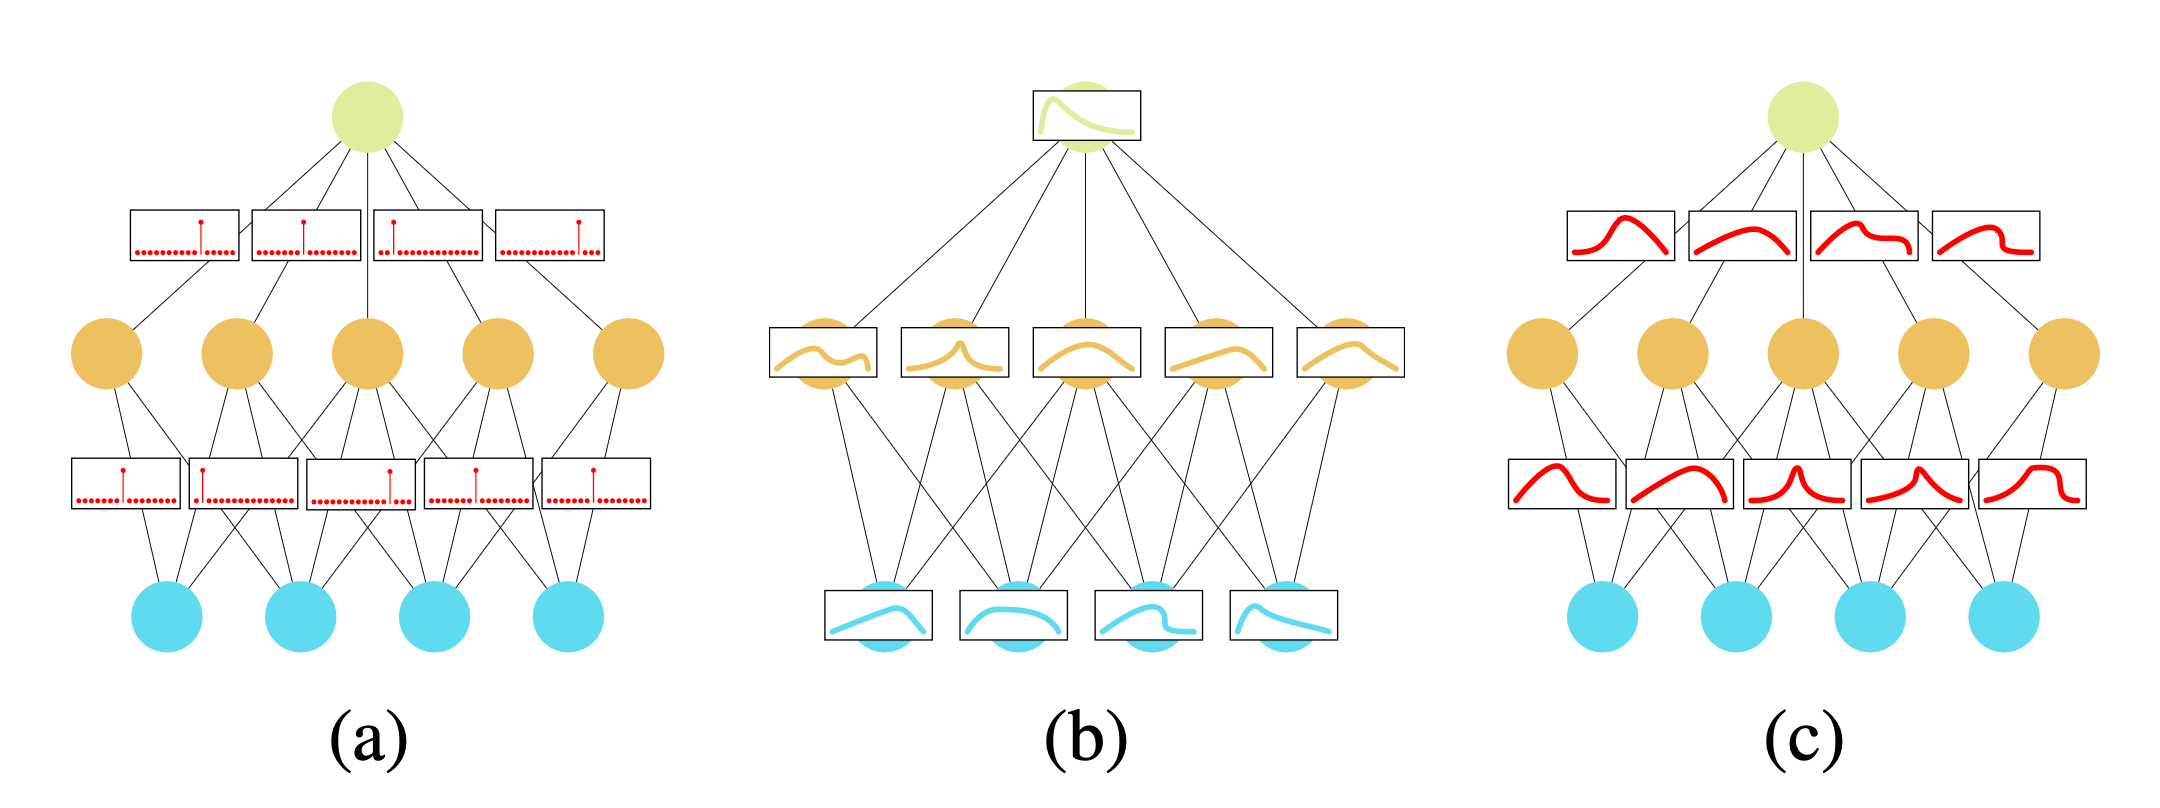
\includegraphics[width=0.9\linewidth]{img/ML/scheme_bnn.png}
    \caption{Illustration for a non-stochastic neural network a), a network with stochastic activations b), and a network with stochastic weights in c). Source: \cite{BNN_review}.}
    \label{fig:ML BNN ilus}
\end{figure}
A Bayesian neural network is defined by a prior distribution over the weights (when they are set to be stochastic), a functional model that forwards the inputs and generates the outputs, and a likelihood model that defines the predictive power of the network $p(y|x,\theta)$. The model weights are update in the presence of data $\mathcal{D}$ according to Bayes' formula
\begin{equation}
    p(\theta|\mathcal{D}) \propto p(\mathcal{D}_y|\mathcal{D}_x, \theta)p(\theta)
\end{equation}
When the model has seen the data, we can use the posterior distribution on the parameters to generate data or make prediction:
\begin{equation}\label{eq:posterior precitive}
    p(y|x,\mathcal{D})=\int_\theta p(y|x,\theta)p(\theta|\mathcal{D}).
\end{equation}
Note that \cref{eq:posterior precitive} weights the predictions by each possible parametrization of the network using the posterior distribution on the weights. In that sense, Bayesian networks can be understood as training an ensemble of networks and then averaging their predictions. Note that ensembles are also a popular technique with classical neural networks \cite{ensemble}. In fact, since the training of a classical network has also stochastic components (the initial weights, shuffling of the data, ...), it is common to train multiple networks with different initialization seeds and weights their predictions, much tend to outperform even the best-performing network.

Let us illustrate how a committee of networks can outperform even a top-performer network. Suppose we train 3 independent networks $A,B,C$ for a classification task with two classes, and that they all have the same error probability $p$. In an exercise of pure democracy \footnote{“I love democracy. I love the Republic”, Senator Palpatine.}, consider a classifier $D$ who picks the class with the majority of votes. Since $D$ is wrong if and only if at most one of the classifiers is wrong, the probability of error for $D$ is (considering $p\to 0$)
$$p^3-3(1-p)^2 =\mathcal{O}(p^2),$$
and hence $D$ outperforms $A,B$ and $C$.


\subsection{Hyperparameter selection}\label{sec:optuna}
The performance and convergence properties of a deep learning model are highly sensitive to its precise architecture, and hence, to the \emph{hyperparameters} that control the latter: number of layers, the exact type of layers (convolutional, dense,...) and other auxiliary parameters that influence the training process. The optimal set of hyperparameters are the ones that produces the best-perfoming model on unseen data. There are three main difficulties when choosing hyperparameters. Firstly, it is not obvious a priori how modifying a certain parameter will affect the performance of a model. For example, if we add an extra layer to a network, will that improve expressivity and performance or will it lead to overfitting? This is a consequence of the low interpretability of deep learning models. Secondly, evaluating the performance of a model requires training it, which is computationally expensive. Finally, there are possibly an infinite number of possible architectures to explore.

Many Python APIs implementing routine to find optimal hyperparameters exists. They include state-of-the-art algorithms for exploring the hyperparameter space, selecting which parameters to explore, and early-stopping the evaluation of unpromising trials. In this work we use \texttt{OPTUNA} \cite{optuna_2019}, which a Python optimization API, to select the appropriate set of hyperparameters for our deep learning models. \texttt{OPTUNA} implements a wide variety of searching algorithms to explore the hyperparameter space. Among those strategies, we can choose a naive grid search, where the user defines a grid over the hyperparameter space, and all possible combination are tested and ranked in a sequential order. \texttt{OPTUNA} can also implement a random search, which randomly selects the next trial over a grid. However, \texttt{OPTUNA} also implements more complex searching algorithms. The default search strategy is the \emph{Tree-structured Parzen Estimator} (TPE) approach. TPE is designed to maximaze the expected improvement when selecting a new sample. If we have already explored a set of points $x$, the expected improvement (EI) for a new trial $y^*$ is defined as
\begin{equation}\label{eq:expected imp}
    \begin{aligned}&\text{EI}_{y^*}(x)=\int_{-\infty}^{y^*}(y^*-y)p(y|x)dy=\int_{-\infty}^{y^*}(y^*-y)p(x|y)\frac{p(y)}{p(x)}dy\end{aligned},
\end{equation}
where we are assuming a one-dimensional problem for clarity, and $p(y|x)$ represents the probability of chossing a trial $y$ having observed $x$, as obtained from the searching algorithm. TPE optimizes \cref{eq:expected imp} by using the following routine \cite{TPE}:
\begin{enumerate}
    \item We initiate a set $\mathcal{D}$ of explored trials with $N_i$ parameters and compute their performance.
    \item $\mathcal{D}$ is split as $\mathcal{D}=\mathcal{D}^l \cup \mathcal{D}^g$ in the top $\gamma$ performers (a common value is $\gamma=0.2$) $\mathcal{D}^l$ and the lower performers $\mathcal{D}^g$.
    \item We fit a two Gaussian mixtured distributions to $\mathcal{D}^l$, l(x) and to $\mathcal{D}^g$, g(x). This is a Kernel Density Estimaton (KDE) for the distribution of both sets. See \cref{fig:ML TPE} for an illustration of this step.
    \item The new trial parameters are selected and added to $\mathcal{D}$ to maximize $l(x)/g(x)$. In practice, this can be done by generating $N_s$ samples from $l(x)$ and then maximizing $l(x)/g(x)$ over those samples.
\end{enumerate}



\begin{figure}
    \centering
    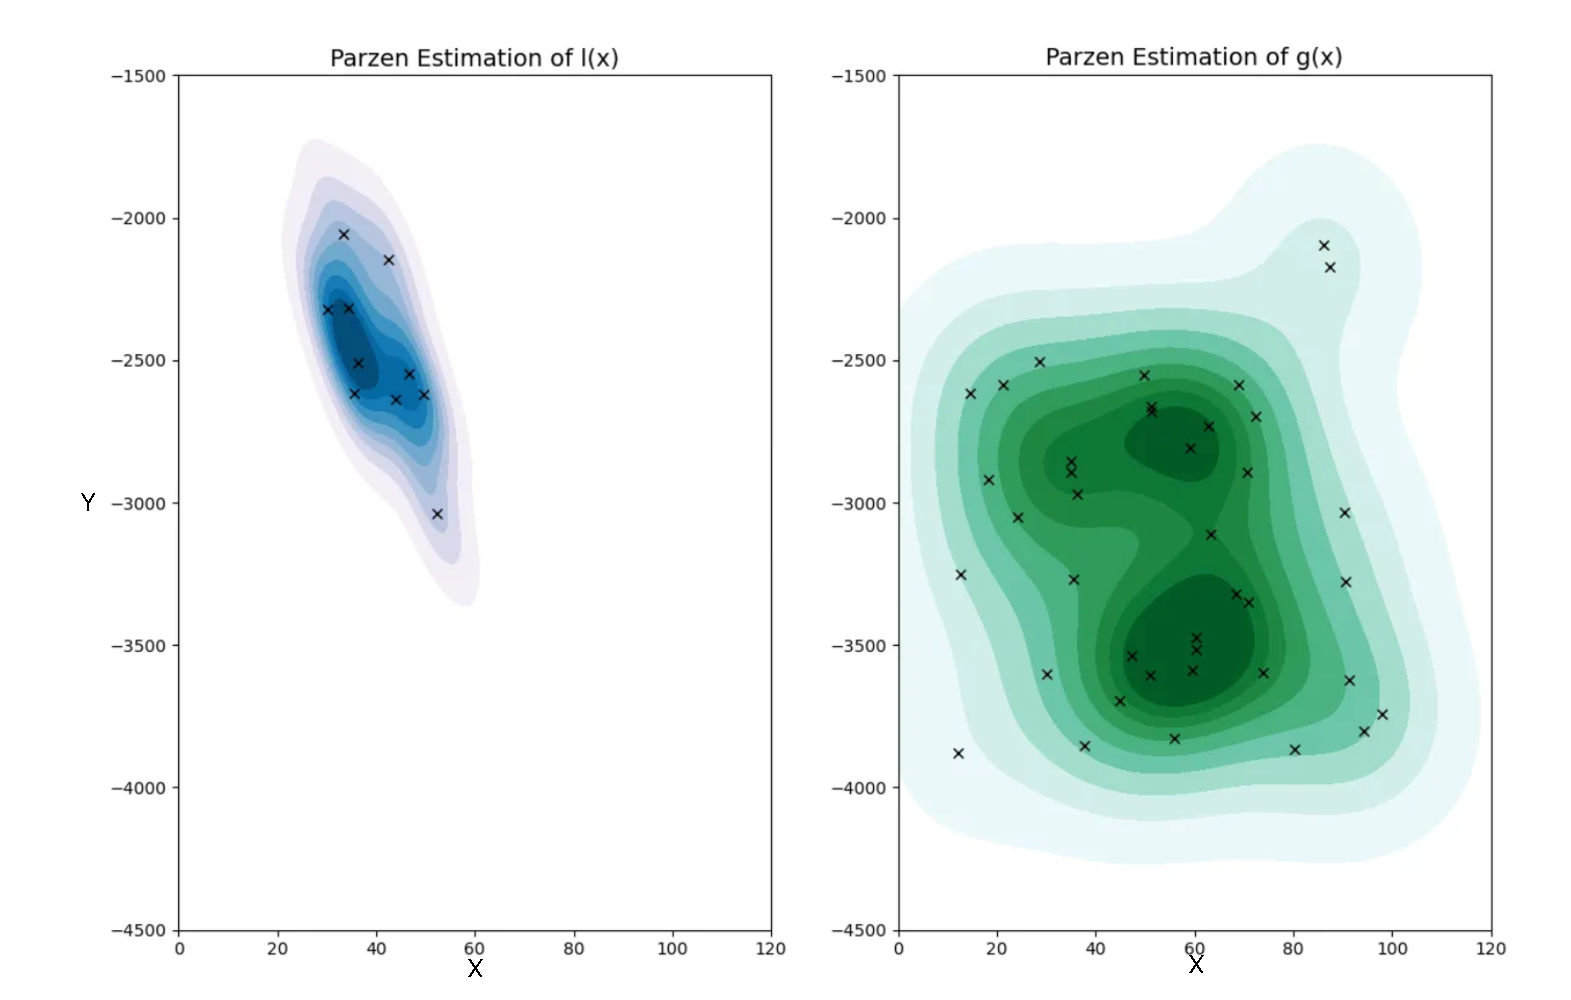
\includegraphics[width=0.6\linewidth]{img/ML/Parzen.pdf}
    \caption{Example DE estimation for the distribution $l(x)$ and $g(x)$ used in the TPE algorithm.}
    \label{fig:ML TPE}
\end{figure}

We can easily show that the TPE routine maximizes the expected improvement \cref{eq:expected imp}.
Firstly, note that $\gamma=p(y<y^*)$ and that $p(x)=\int p(x|y)p(y)dy=\gamma l(x) +(1-\gamma) g(x)$. Furthermore, if $y<y^*$, we have that 
$p(y|x)=l(x)$, and hence,

\begin{equation}
    \int_{-\infty}^{y^*}(y^*-y)p(x|y)p(y)dy=\ell(x)\int_{-\infty}^{y^*}(y^*-y)p(y)dy=\gamma y^*\ell(x)-\ell(x)\int_{-\infty}^{y^*}p(y)dy.
\end{equation}
We conclude that 
\begin{equation}
    \text{EI}_{y^*}(x)\propto \left(\gamma+\frac{g(x)}{\ell(x)}(1-\gamma)\right)^{-1},
\end{equation}
and so we need to maximize $l(x)/g(x)$, as previously discussed.




\subsection{Loss function and training}
In this section, we further detail to training process of a deep learning model, and describe the alhorithms that will be used to train our model.
As we have already discussed in section \ref{sec: dataset}, the goal of our model is the minimize the generalization error:

\begin{equation}
    \varepsilon =\mathbb{E}_F[\mathcal{L}(Y,\hat{f}(X|\mathcal{D}_T))].
\end{equation}
The loss function $\mathcal{L}$ should be choosen to encourage the model to produce realisitc outputs. For regression, where the goal is to estimate an output tensor $Y$ from an input $X$, typical choices include the usual Euclidean norm or the absolute difference:

\begin{equation}\label{eq:euclidean norm}
    \mathcal{L}(Y,\hat{Y})=\sum_i |\hat{Y}_i-Y_i|^p, p=1,2,
\end{equation}
where $\hat{Y}$ is the model prediction. This choise of loss function is minimzed when the model correctly predicts the target tensor.
An important information to note is that \cref{eq_ch3:global_loss} is generally unkown, since we don't have acces to all the possible realizations of the data, but only to a limited training dataset. As a consequence, we typically minimize the loss function computed on small samples of the training data, called \emph{batches}, by averaging the loss over all samples in the batch. Observe that then, computing the average loss over a large batch will yield a closer approximation to the true loss function. The training process then uses these estimations of the loss to update the network parameters, $\theta$, using techniques that involve the computation of the loss gradient. This process is normallh repeated multiple times over the training dataset. Each time the model sees the whole dataset is knwown as an \emph{epoch}. A training loop with $N_e$ epochs and batches of size $B_s$, with $N_b$ batches, can then be written as:

\begin{algorithm}
    \caption{Classical deep learning training loop}\label{alg:training loop}
    \begin{algorithmic}
    \While{$\text{epoch} <N_e $}
        \While{$\text{batch} <N_b $}
        \State $\text{Loss}\gets \frac{1}{B_s}\sum_i\mathcal{L}(\hat{Y_i},Y) $
        \State Compute $\nabla_\theta (\text{Loss})$
        \State Update $\theta \gets \theta(\nabla_\theta (\text{Loss}))$
        \EndWhile    
    \EndWhile
    \end{algorithmic}
    \end{algorithm}

In algorithm \ref{alg:training loop} there are two main steps we have not specified. Firstly, the comoutation of $\nabla_\theta (\text{Loss})$. This is trivial from the mathematical viewpoint, but it is not trivial to implement\footnote{Note that this is purely a computer science problem.}. Most APIs implement a \emph{backpropagation} algorithm for this step that we will not discuss here\footnote{\url{https://www.tensorflow.org/guide/autodiff}}. The second key aspect of a training loop is using the gradient $\nabla_\theta (\text{Loss})$ to update $\theta$. This step in algorithm \ref{alg:training loop} was repreented by $\theta \gets \theta(\nabla_\theta (\text{Loss}))$. The precise way of using the calcualted loss gradients to update the weights define the \emph{optimizer}\footnote{Note that this is purely a mathematical problem in optimization.}. A naive way to optize the loss at each iteration is to use the most straightforward implementation of \emph{gradient descent}, where the parameters are updated using
\begin{equation}
    \theta \gets \theta - \alpha \nabla_\theta (\mathcal{L}),
\end{equation}
where $\alpha$ is a constant known as the \emph{learning rate}. In general, optimizing the loss function $\mathcal{L}$ corresponds to optimizing a complex (perhaps non-convex) function on a highly multidimensional space, with millions or billions of parameters. As a consequence, naive gradient descent might not be the best-performing optimizer. Additionally, recall the loss $\mathcal{L}$ calculated for every batch is just an approximation of the global loss \ref{eq_ch3:global_loss}. The batch size determines how accurate the computed gradient is. Calculating the loss over all possilbe data points would yield the exact gradient. On the opposite extreme, calculating the gradient on a single data point would generate a biased gradient, and lead to a noisy gradient descent. The loss function can also have a complex strucuture. In the literature, a multitude of optimizers that improve and generlize the naive gradient descent exist. In this work, we use \emph{Adam} \cite{adam}. Adam is a first-order momemtum-based optimizer. Adam uses recursive update of the first and second moment of the gradient to update the learnable parameters. The Adam algorithm reads as follows:

\begin{algorithm}
    \caption{Adam optimizer}\label{alg:adam}
    \begin{algorithmic}
            \Require $\alpha$ : Learning rate
            \Require $\beta_1, \beta_2$: Moment decay rates
            \Require $f(\theta)$: Target function
            \Require $\theta_0$: Initial parameters
            \Require $\varepsilon$: Numerical tolerance constant
            \State $m_0 \gets 0$: Initialize first moment
            \State $v_0 \gets 0$: Initialize second moment
            \State $t \gets 0$: Initialize time
            \While{$\theta_t$ not converged}
                \State $t \gets t+1$
                \State $g_t \gets \nabla_\theta f(\theta_{t_1})$: Get gradient
                \State $m_t \gets \beta_1 m_{t-1}+(1-\beta_1)g_t$: Update first moment
                \State $v_t \gets \beta_2 v_{t-1}+(1-\beta_2)g_t^2$: Update second moment
                \State $m_t \gets m_t/(1-\beta_1^t)$: Correct first moment bias
                \State $v_t \gets v_t/(1-\beta_2^t)$: Correct second moment bias
                \State $\theta_t \gets \theta_{t-1}-\alpha m_t/(\sqrt{v_t}+\varepsilon)$: Update parameters
            \EndWhile


    \end{algorithmic}
\end{algorithm}
Adam differs in two key features with respect to the naive gradient descent. Firstly, it includes two decay constants $\beta_1$ and $\beta_2$ used to include information about the past state of the optimization into the next current step. Since typical values are $\beta \sim 0.9$, recent gradient values contribute more to the current step update than older ones, but the inclusion of a momentum term allows the optimization to potentially escape local minima. Secondly, Adam includes a term $v_t$ to account for the second moment in the gradient estimation. The running averages in Adam can potentially help to navigate noise functions by smoothing the local gradient.


Most current deep learning implementations are deployed or trained using HPC infrastructure. This becomes a necessity when training on large datasets. A quickly deployable way of paralellize training, and which requires minimal code modification is known as \emph{Synchronous Distributed Training}. Synchronous Distributed Learning aims to harvest to computational power of multiple machines (GPUs,...) in the training stage by having different workers perform parallel calculations in a single batch. This can be done, for instance, by splitting the batch and sending each part to a different worker. In this work, we use the TensorFlow implementation \texttt{tf.distribute.MirroredStrategy}. This training strategy mirros the model and its parameters in every worker (for instance, in every GPUs), slices the training batch and distributes them accross all workers. Each worker then calculates the loss and gradient in the corresponding batch slices. The gradient is then aggregating before updating the parameters and moving onto the next batch.

\begin{figure}
    \centering
    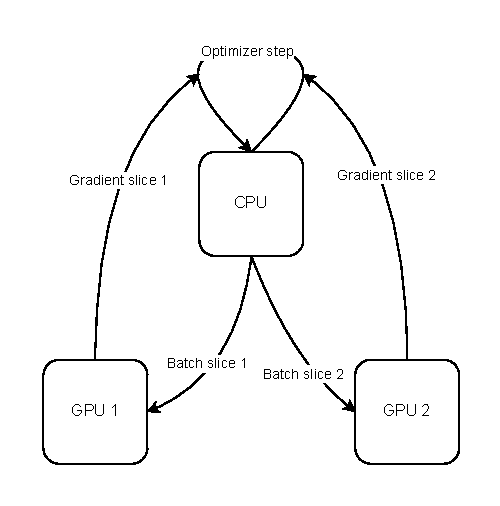
\includegraphics[width=0.6\linewidth]{img/ML/mirror_training.drawio.pdf}
    \caption{Distributed mirrored learning strategy with two workers (GPUs) and a CPU agregating the gradient and updating the model parameters.}
    \label{fig:ML mirror training}
\end{figure}

\section{Workflow implementation: Recovering IGM conditions from the Lyman-alpha forest }
This section describes the deep learning implementation used in this work and built in the ideas that have already been introduced regarding machine learning. The code used is largely based on \cite{nasir2024deep} with very minor modifications and is avaible at \url{https://github.com/nicenustian/bh2igm} and based on TensorFlow and TensorFlow Probability.


The ultimate aim is to use a Bayesian neural network to recover the IGM gas density from an input Lyman-$\alpha$ skewer. Note that this is essentially equivalent to invert Equation \ref{eq:lyman opacity}, which describes the Lyman-$\alpha$ opcaity as a function of the IGM gas conditions. As we have already discussed int \ref{sec: optical depth weighted}, we will work int the optical depth-weighted space. This avoids two main potential difficulties in the anaylisis. Firstly, by working in this new space, the network will not have to learn the relation between peculiar velocities and the Lyman-$\alpha$ opcaity, which simplifies both the architecture design and learning phase. Secondly, it breaks the degeneracy introduced by peculiar velocities, since a shift in the physical space can produce the same opacity as a shift in the velocity space.

We specify the architecure design by the hyper-parameter list found in \cref{table: fiducial architecture}. The global architecure that describe the number and size of the layers is specified by two hyper-parameters. Firstly, the parameter ''Layers per block'' is an integer list whose size is the number of blocks in the network and whose elements are the number of layers in each block. Secondly, the parameter ''Filters per block'' is also an integer list that specifies the number of convolutional filters of the layers for each block. If the architecure is a simple MLP, this parameter does not have any affect. The layers are choosen among a simple densly connected layer (MLP), and convolutional layer (ConvNet) or a residual layer (ResNet). Every feedforward pass through a convolutional or densely connected layer is followed by a batch normalization layer and by an activation function, see section \ref{sec:deep learning archi}. We use the PReLU activation function, wich is a generalization of the ReLU activation with a learnable weight $\alpha$ such that:
\begin{equation}
    \text{PReLU}(x;\alpha)=
    \begin{dcases}
        \alpha x &  , x<0\\
        x & , x\geq 0
    \end{dcases}
\end{equation}
We append the same final block to all three potential architecutres, which consists of a flattening layer transforming the tensor being manipulated to a one-dimensional vector, a dense layer a finally a Gaussian probabilistic layer.
This final block includes the stochastic components of the neural network (hence the name Bayesian). For each target output density pixel the Gaussian layer outsputs a full Gaussian probability distribution parametrized by the expected density and the standar deviation. This standar deviation will later be used as the estimation for the espistemic uncertainty in the network prediction. We illustrate the fiducial architecture in \cref{fig:ML nn architecture}.
\begin{figure}
    \centering
    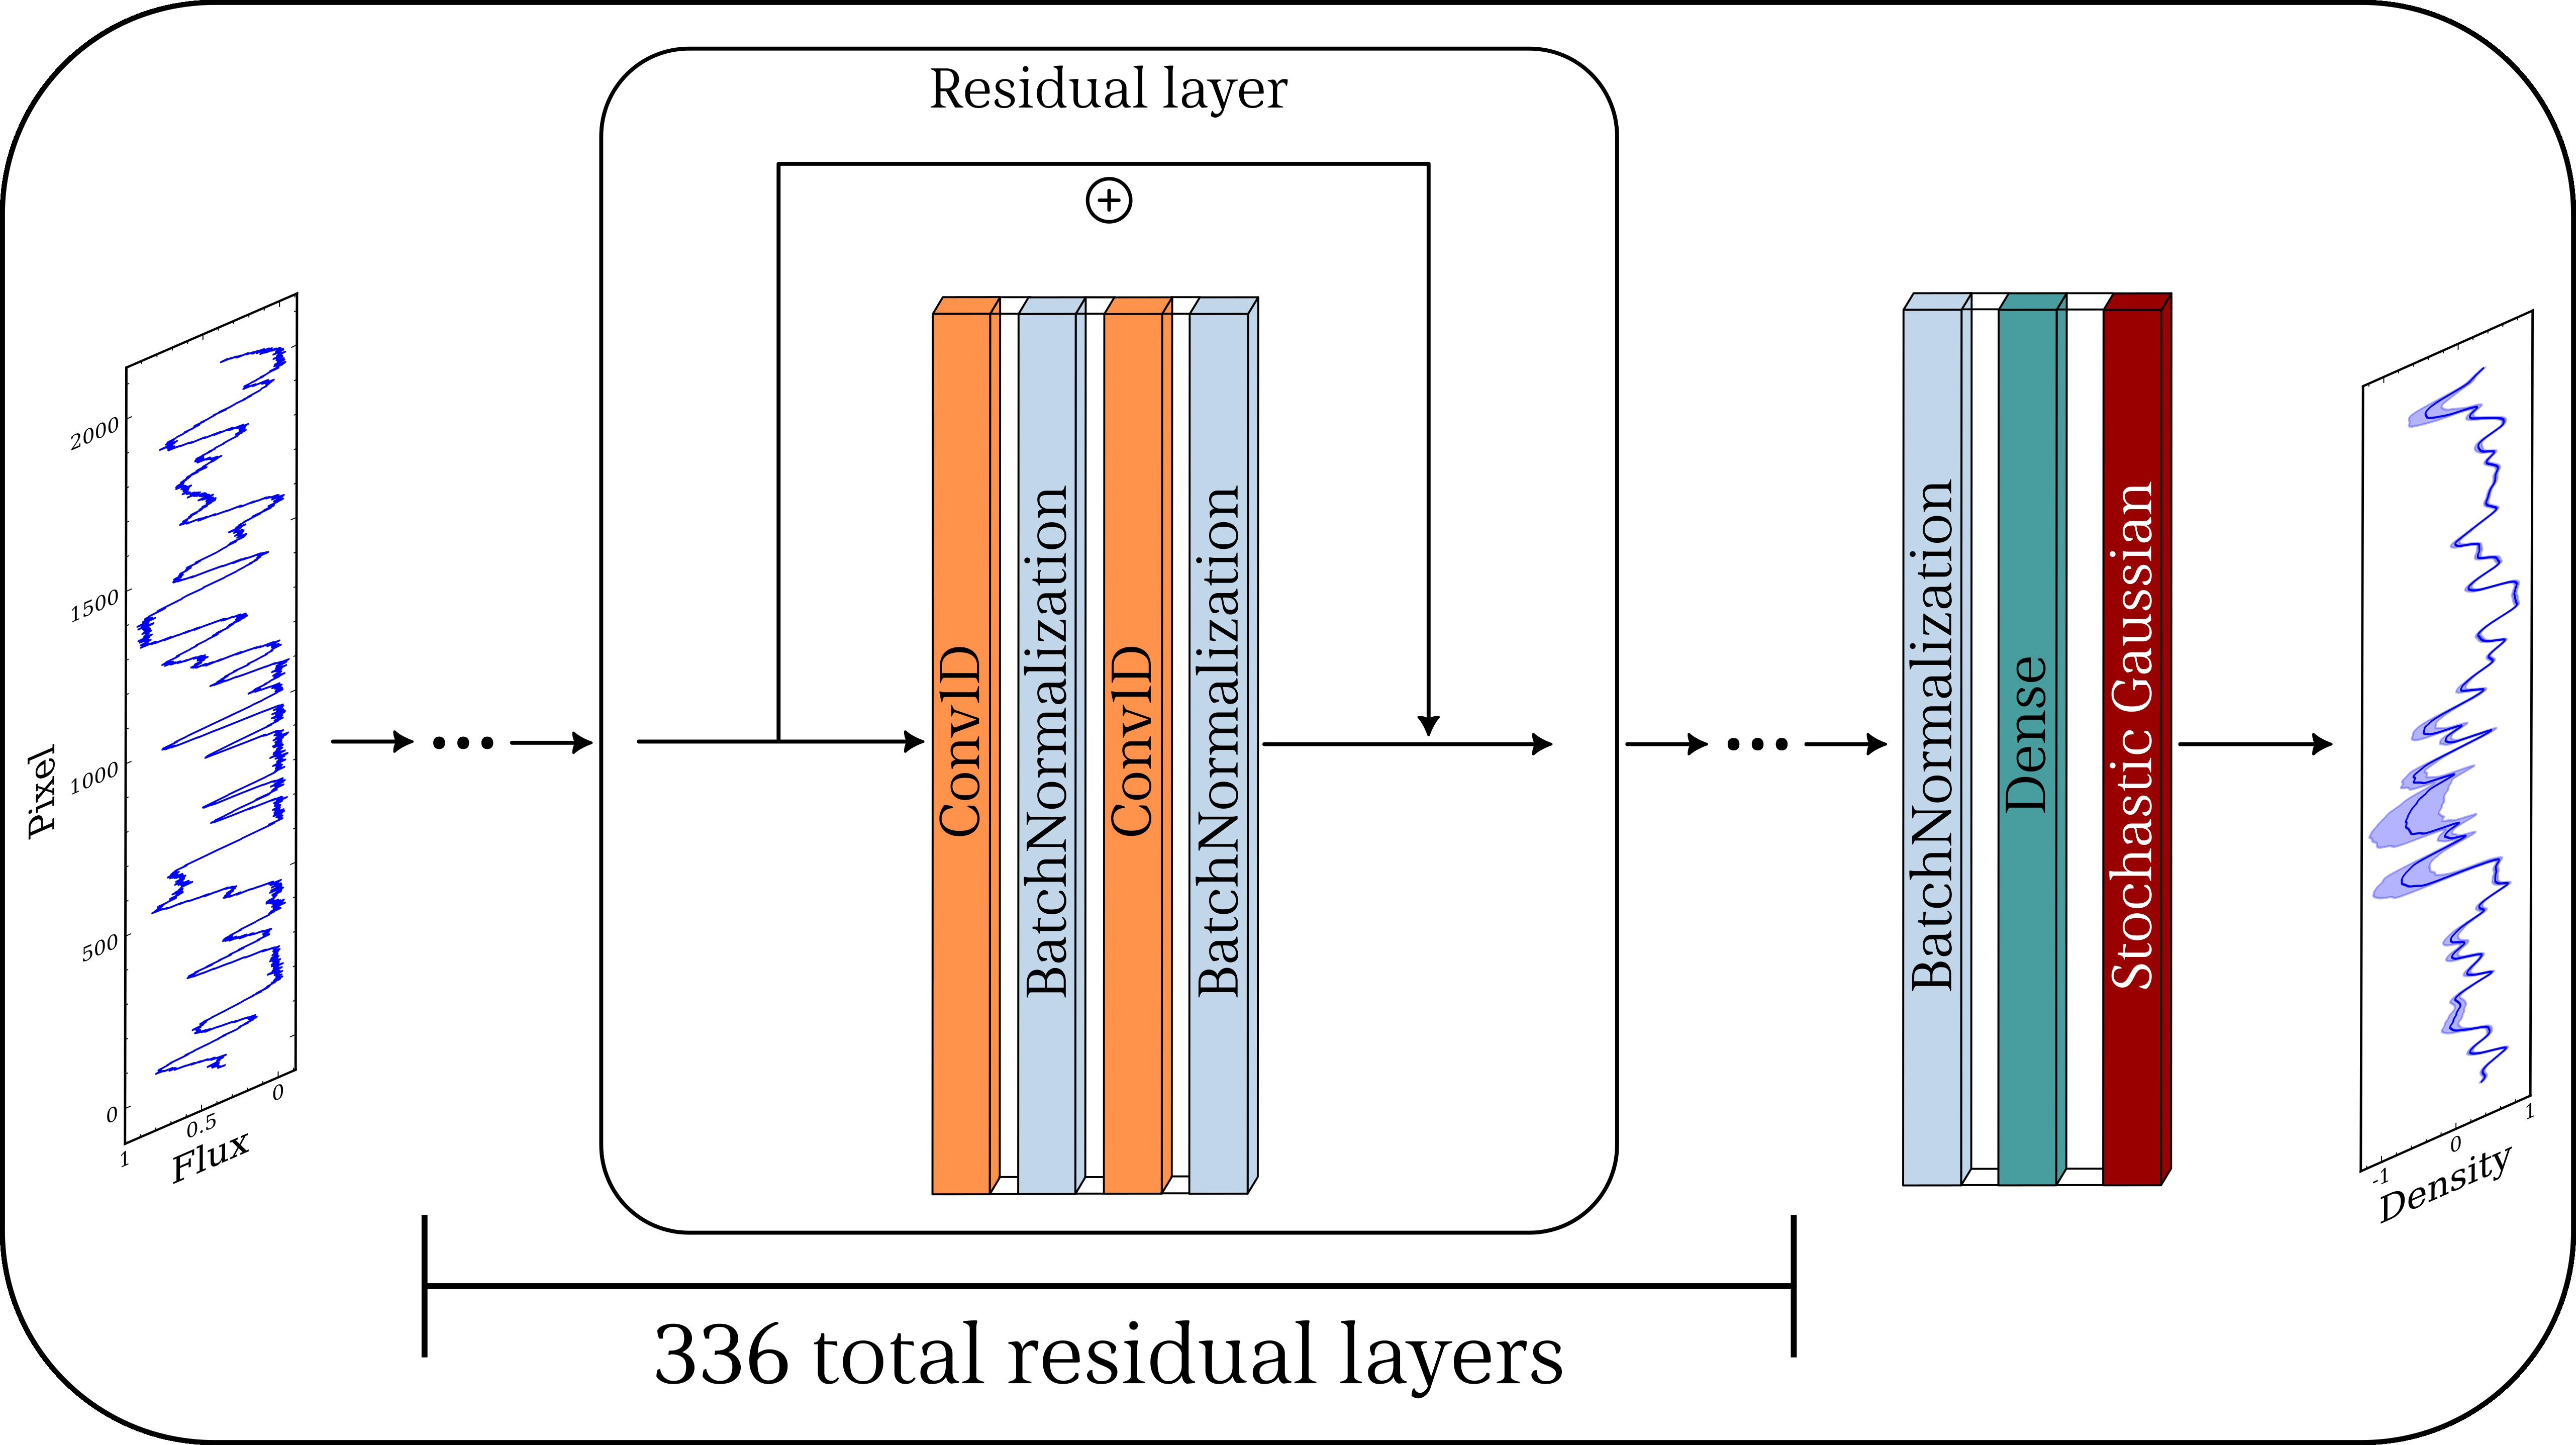
\includegraphics[width=1\linewidth]{img/ML/nn_archi.jpg}
    \caption{Fiducial architecture for our Bayesian neural network trained at $z=4.4$ on the Sherwodd simulation suite. The fiducial parameters can be found in \cref{table: fiducial architecture}.}
    \label{fig:ML nn architecture}
\end{figure}

We optimize the netowork hyper-parameters using \texttt{OPTUNA} as discussed in section \ref{sec:optuna}. Table \ref{table: fiducial architecture} the optimized hyper-parameters and the range considered during the grid search. Note that these values can potentially deppend on the nature of the training dataset, and hence may vary with redshift. In table \ref{table: fiducial architecture} we present the fiducial architecture at $z=4.4$. This optimizating process is automatically carried out whenever the redshift is varied.

For each redshift, we train a different network using the Sherwood simulation suite presented in section \ref{chap:sherwood}. Recall that we consider two training datasets, \texttt{SHERWOOD} and \texttt{SHERWOOD THERMAL}, where the latter includes variations in the thermal parameters and reionization history. See \cite{sherwood_wdm} for more details. The inclusion of thermal parameters will lead to a more robust network when used on unseen real data, but its performance will naturally be lower than the network trained on a single thermal hsitory. We use \texttt{SHERWOOD} for an initial model testing, and \texttt{SHERWOOD THERMAL} for our final anaylisis on real data. 80 \% of the data is used for training, and the rest is used for validation purposes. For reference, the training dataset \texttt{SHERWOOD} with,7 different WDM models has a total size of $\sim 3.5$ GB. We use the Raven\footnote{\url{https://www.mpcdf.mpg.de/services/supercomputing/raven}} HPC cluster at the Max Planck Computing and Data Facility to train our networks. With 4 Nvidia A100 GPUs, a typical training time is $\sim 1$ hour, depending on the model's exact architecture and number of parameters.


\begin{table}
    \centering
    \begin{tabular}{|c|c|c|c|}
        \hline
        Hyper-parameter&Min.  &Max.  &Best value \\
        \hline
        Layers per block (int)& 1 & 4 & [1, 2, 4 ,4] \\
        $\log_2$(Filters per block) (int)&$1$  &$5$  &  [4, 5, 5, 5] \\
        Number of blocks (int)&1  &4  &4 \\
        $\log_2$(Batch size) (int)&3  &8  & 3 \\
        Learning rate ($\log_s$, float)&$10^{-4}$  & $0.1$  &0.004937 \\ \hline
        Network (MLP, ConvNet, ResNet)&...  & ... &ResNet \\
        \hline
    \end{tabular}
    \caption{Hyper-parameter grid search for the fiducial model at $z=4.4$. ``$\log_s$'' indicates the parameter is sampled in the log domain. ``Int'' and ``float'' mean they are sampled as integers or floats, respectively.}
    \label{table: fiducial architecture}
\end{table}


The network's input consist of a Lyman-$\alpha$ flux skewer, and the network's output consists of the mean density and standard deviation at each pixel. The labelled training data consists of individual Lyman-$\alpha$ flux skewers with their associated density optical depth-weighted density field, $(F,\log(\Delta_\tau))$. For each labelled training pair, the loss function is taken to be the negative log-likelihood (NLL) for the normal distribution that the network parametrizes:

\begin{equation}\label{eq:our loss}
    -\log\mathcal{L}=\frac{1}{N}\sum_{{\mathrm{i}}}\left((Y_{{\mathrm{i}}}-Y_{{\mathrm{i},\mathrm{pred}.}})^{2}/\sigma_{{\mathrm{i},\mathrm{pred}.}}^{2}+\log(\frac{1}{\sigma_{{\mathrm{i},\mathrm{pred}.}}^{2}})\right),
\end{equation}
where the sum runs over all skewer pixels,$Y_i$ is the real density at pixel $i$, $Y_{{\mathrm{i},\mathrm{pred}.}}$ is the predicted expected density and $\sigma_{{\mathrm{i},\mathrm{pred}.}}^{2}$ the predicted standard deviation.

The input skewers are processed as follows. Firstly, the input flux is rebinned into a target number of pixels to match the real data that will be used. Downsampling is done by taking the avarage flux over nearby pixels, while upsampling is done by appending to every pixel a copy of itself. The flux is then convolved using a gaussian kernel to simulate a given instrumental resolution. In most of our analysis the resilution is taken to be $6$ km/s, in accordance with state-of-the-art spectrographs, such as UVES \cite{UVES}. During training, the training data is stacked and randomly shuffled to ensure a correct mixing and representativity of the models. Lastly, we process the reescale input optical depth to match the observed mean flux at the considered redshift \cite{Becker_mean_flux}.
The training data is augmented on-the-fly in two ways. We first roll the input spectra by application translations, this helps the network learning dynamical features, independently of their positions. We also add random uncorrelated gaussian noise to simulate a finate signal-to-noise ratio (SNR). The default SNR per pixel used for testing purpises is 50. When applying our methods to real-data, the network is retrained using a noise model for each target object.


We use the Adam optimizer with fixed moment decay rates as implementation in the TensorFlow API and a learning rate set by the Optuna grid search. The training is evaluated using two main metrics: the loss function NLL, and the mean absolute error, MAE, defined as the Euclidean norm \ref{eq:euclidean norm} in with $p=1$. To prevent over-fitting, the network parameters are only updated if the NLL loss improves on the validation split of the data. A policy to halve to learning rate if there is no loss improvement in the test set for 10 epochs is also included. This is the most straightforward adaptation of an adaptive learning rate. Figure \ref{fig:ML learning curve} shows the evolution of the NLL and the MAE on the validation split during training for our fiducial architecture at $z=4.4$ and the \texttt{SHERWOOD} suite. It is interesting to note that while the MAE is always positive by definition, negative valueso of the NLL are consistent with its definition. Figure \ref{fig:ML learning curve} demostrates that, for our problem, the network training coverges in $\sim 100-150$ epochs. Recall that we always work with $\log(\Delta_\tau)$, which also serves as a regulatization step with respecto to the density.


\begin{figure}
    \centering
    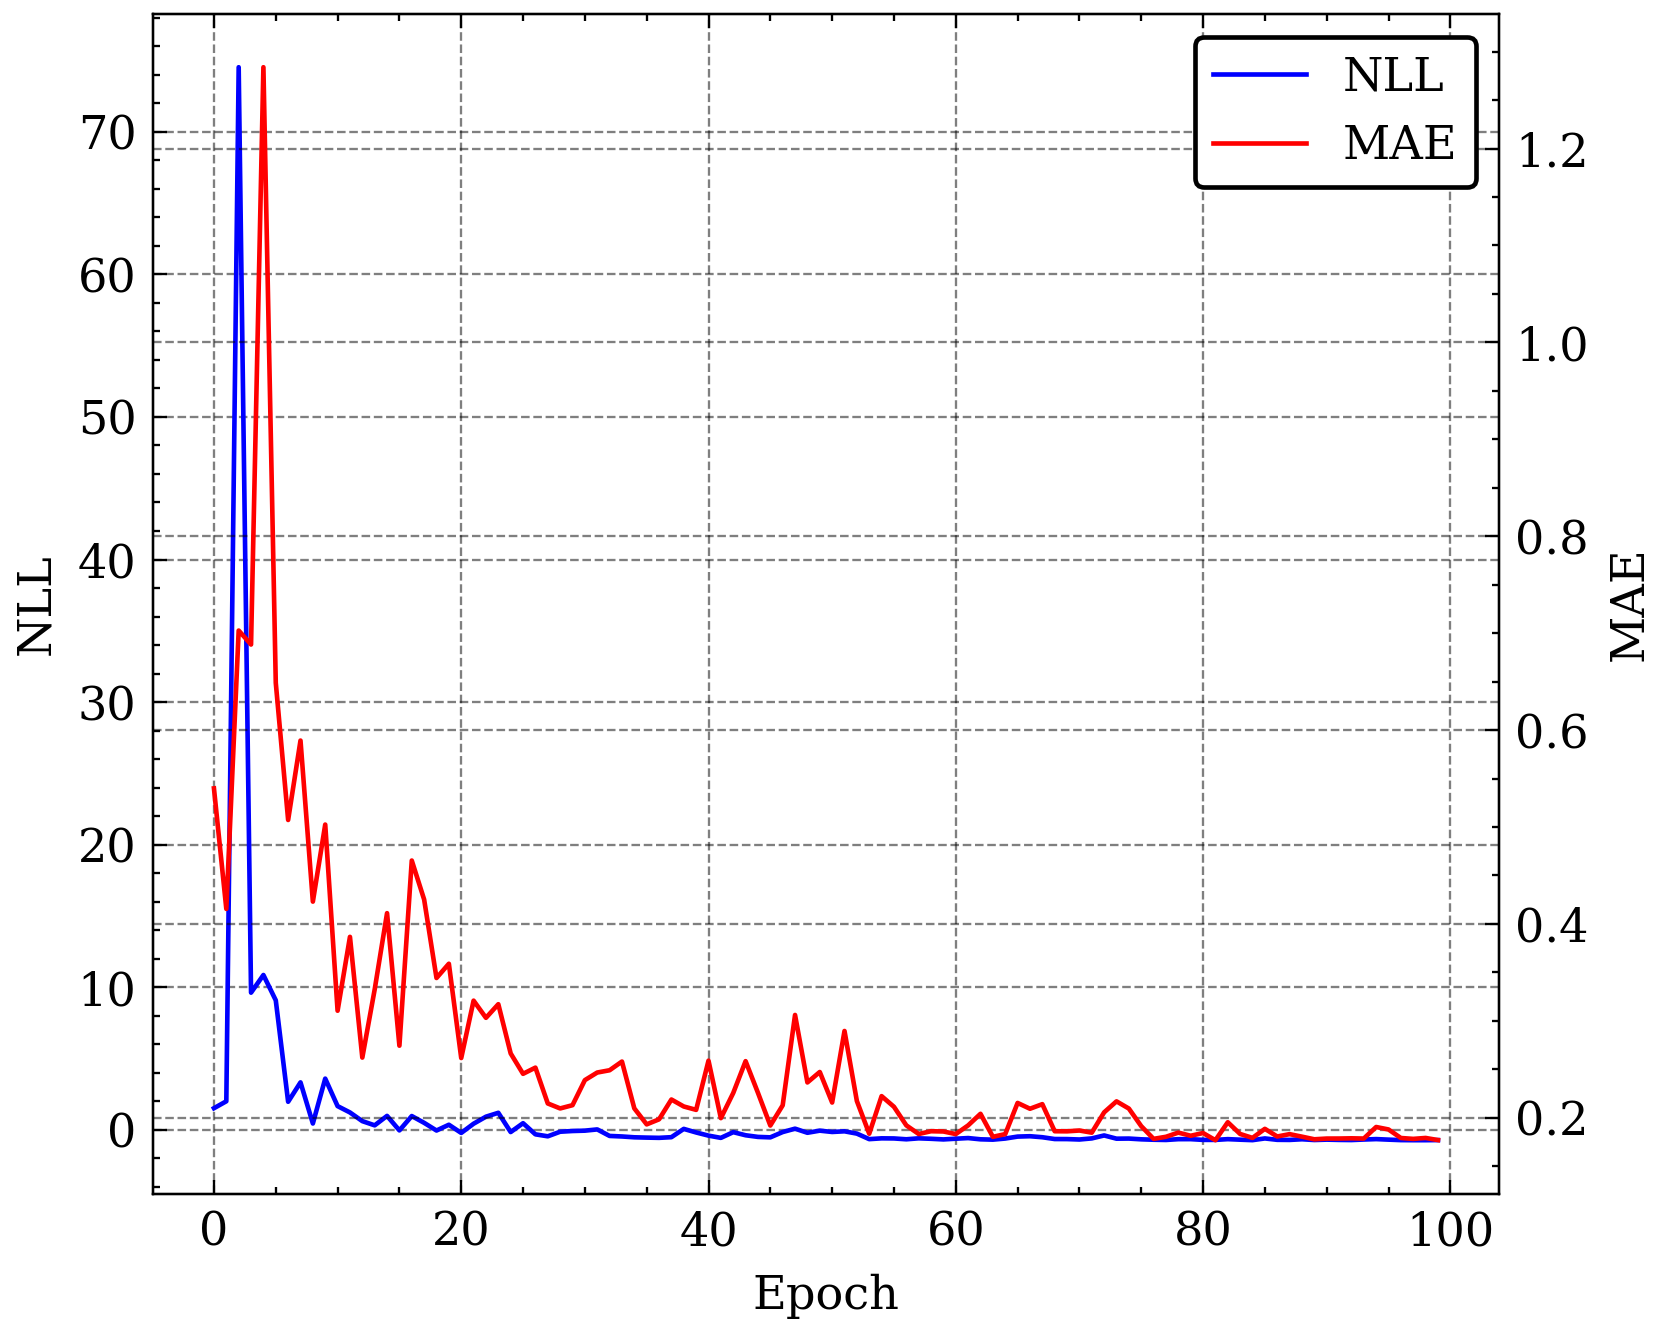
\includegraphics[width=0.7\linewidth]{img/ML/learning_curve.png}
    \caption{Learning curve for our fiducial architecture at $z=4.4$ on the \texttt{SHERWOOD} dataset. The figure shows the NLL and the MAE on the validation split as a function of the epoch.}
    \label{fig:ML learning curve}
\end{figure}

In \cref{fig: example_recovered_skewer} we show an example 20h$^{-1}$cMpc  Lyman-$\alpha$ validation skewer from the \texttt{SHERWOOD} dataset. The top panel shows the input flux to the network. The bottom panel shows the true $\Delta_\tau$ density fields, the (mean) recovered densities and the $1\sigma$ envelope predicted by the Bayesian network. Note that, in the spectral regions with large features and variations in the flux, the predicted mean density closely follows the true field. In those regions, there is enough physical information for the network to accurately recover $\Delta_\tau$. In contrast, in the saturated regions with low flux, the noise dominates, and the network predicts larger uncertainties (observe, for instance, the saturated region in Figure \ref{fig: example_recovered_skewer} around 8h$^{-1}$cMpc). This should be regarded as a strength of Bayesian netoworks, since they are able to accurately detect and make explicit situations where the predictions should not be trusted. To minimize the mean error in regions where the network cannot make accurate preditions, note how there is a bias towards quasi-constant mean prediction. This is visible around 8h$^{-1}$cMpc, where the true density has a steep increasing profile, and the predition has an almost constant u-shaped profile.

\begin{figure}
    \centering
    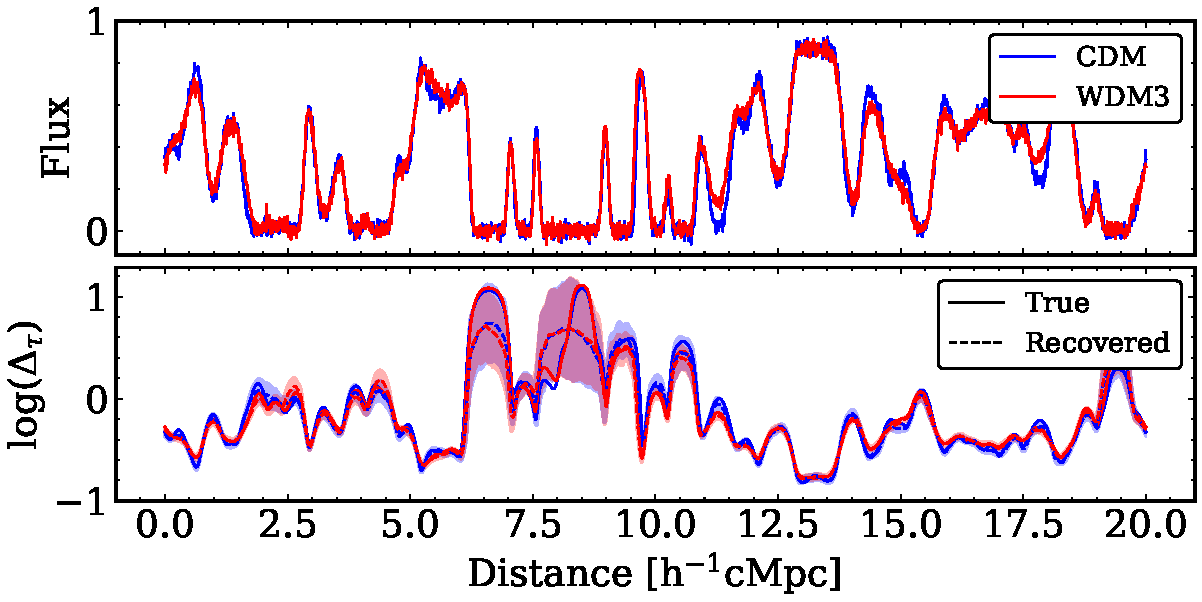
\includegraphics[width=0.99\linewidth]{img/ML/skewer.pdf}
    \caption{An example 20h$^{-1}$cMpc Lyman-$\alpha$ validation skewer for the CDM and WDM3 Sherwood models. The top panel shows the input flux to the network. The bottom panel shows the true $\Delta_\tau$ density fields, the (mean) recovered densities and the $1\sigma$ envelope predicted by the Bayesian network.}
    \label{fig: example_recovered_skewer}
\end{figure}
On the \texttt{SHERWOOD} validation split, the network reaches a $1\sigma$ accuracy of $79\%$, meaning that $79\%$ of the pixels are correctly predicted within $1\sigma$. Note that this is a larger accuracy that expected from purely normally-distributed densities.




 ,.... violin...compare thermal models and non thermal










\section{Recovered field statistics and uncertainties}\label{sec:recovered statistics}
Once we have a machinery to recover the IGM density from a Lyman-$\alpha$ skewer, we would like to use this density field information to do statistical inference on the physical parameters of interest. In this work, since the WDM mass directly affects the matter distribution of the Universe (see Figure \ref{fig:villasenor_wdm}) we would like to infer the WDM masses from the recovered $\Delta_\tau$ field. Now, note that the exact $\Delta_\tau$ field of a skewer, such as the one shown in Figure \ref{fig: example_recovered_skewer}, not only depends on a set of physical paramters (WDM mass, temperat,...) but also on the initial conditions or equivalently, the random seed in the cause of a simulation. As a consequence, we will not compare densities on a sightline by sightline basis, but rather compute and comapre agregatted statistics of the fields over multiple realizations that capture global statistical properties, and not simulation-specific characteristics. Statistics that have been amply tested in the literature are the Power Spectrum (PS), the Probability Distribution Function (PDF), the curvature, or the autocorrelation function (see
\cite{Gaikwad_2021} and \cite{wolfson2023forecastingconstraintshighzigm} for more details). In this work we will focus on the $\Delta_\tau$ PDF. In section \ref{sec:IMNN} we will address the optimiality of this choice. 

ADD bootstrapping and PDF OF PDF
ADD MATRIX CORR and resampling and recoveries using finite skerwers

\begin{equation}\label{eq: residuals}
    r_i=\frac{\Delta_{\tau,i}-\mu_i}{\sigma_i}
\end{equation}



PDF:
\begin{equation}\label{eq:PDF of PDF}
    p(\lambda |f(x),N )\propto \frac{\Gamma(N+1)}{\Gamma(N\lambda+1)\Gamma(N-N\lambda+1)} f(x)^{N\lambda}(1-f(x))^{N(1-\lambda)}
\end{equation}

























\section{Model interpretability and limitations}
Deep learning models tend to have, by definition, numerous parameters. As a consequence, giving an interpretation for individual model parameters is far from being a trivial task. On top of the large number of parameters, the nonlinearities and the potentially biased and uncomplete datasets can lead to complex training behaviors. In that regard, deep learning models have classically been regarded as ``black-box'' models. They are often more accurate than simpler statistical models, but lack explainability. Great efforts have been recently made in undertanding the learning dynamics of neural networks \cite{shwartzziv2017opening}, \cite{buhrmester2019analysis}, \cite{explaiNN}.
Due to the complexity of this interpretation task, here we choose to only give a qualitative analysis of some aspects that can help gain intuition on how the newtork operate internally.

\subsection{Saliency analysis}
Although many open-source libraries, such as \textit{Captum}\footnote{https://github.com/pytorch/captum}, implement popular methods for deep learning model visualization and interpretation, in this work we use TensorFlow's built-in'differentiation capabilities. In particular, we use Automatic Differentiation to compute the \textit{saliency} score of the model, defined as the gradient of the model output with respecto to the model input. As a consequence, for every target density pixel, the saliency score measure which flux pixel variation contributes the most to a change in density. Saliency is a simple socre giving us insights into how the model uses flux to recunstruct densities. Additionally, note that calculating such gradients do not requeire any numerical finite diffrence approximation, since TensorFlow's GradientTape class can build an exact computational graph with all the operations performed on the input flux. Saliency maps are a popular technique in applied science to explore deep learning model. In fact, in many physics reachearch articles, it tends to be the only tool used for this purpose. This highlights the need to develop more robust and easily-deployable frameworks for deep learning models.

The saliency at density pixel $i$ and input flux pixel $j$ is simply

\begin{equation}
    \text{Saliency}(i,j) = \frac{\partial  \mu_i}{\partial f_j}.
\end{equation}

Figure \ref{fig: saliency} shows the saliency profile averaged over all output density pixels. This gives a global average metric on the relevant flux pixels to predict the density at a certain pixel. The typical saliency ``length'', that is, the typical number of pixels from the pixel center that are useful to predict its density is $\sim 30$. Since at redshift $z=4.4$ our pixel scale on the \texttt{SHERWOOD} data is $1.3$ km/s, we obtain that in velocity space a window of $\sim 40$ km/s is needed to recover the density at a pixel. This particular dynamic is coherent with the underlying physical process, which is a strong robustness sign of our machine learning model. In fact, for the typical IGM gas in the \texttt{SHERWOOD} suite, the Lyman-$\alpha$ absorbtion cross-section profile has a typical scatter of (see Equation \ref{eq:lyman opacity} $ b(T) \sim 20$ km/s.


\begin{figure}
    \centering
    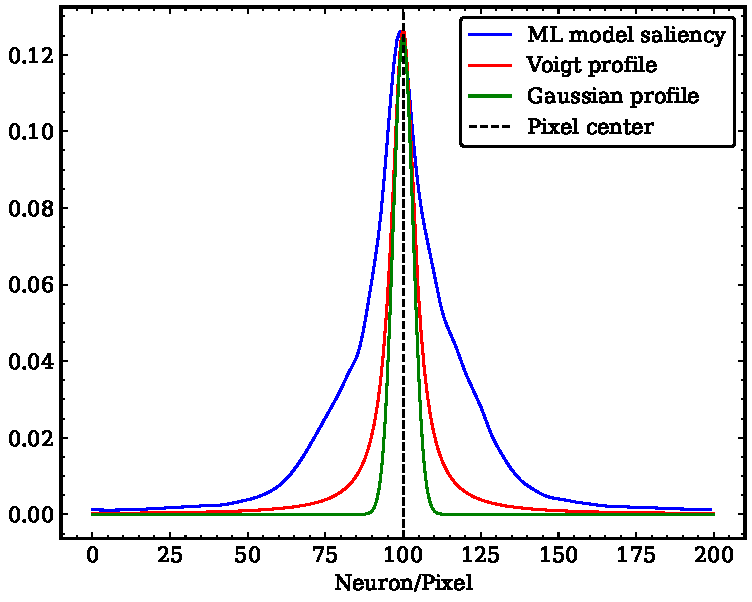
\includegraphics[width=0.6\linewidth]{img/ML/saliency.pdf}
    \caption{Saliency of the CDM and WDM3 Sherwood network at 8h$^{-1}$cMpc Lyman-$\alpha$ flux.}
    \label{fig: saliency}
\end{figure}



\subsection{Covariate shift}
As we have already mentioned when discussing Figure \ref{fig: example_recovered_skewer}, saturated regions lead to larger uncertainties in the network's predictions, reflecting the fact that noise dominates over the physical signal. Observe again the saturated region around 7h$^{-1}$cMp and 8h$^{-1}$cMp in Figure \ref{fig: example_recovered_skewer}. Both of these regions have completly different density profiles, but the network predicts the same u-shape profile with a similar peak density. This peak density is slighlt above the mean density in the simulation box and is similar for the CDM and WDM3 models. We can interpret this as the network leaning a unique mean ``high-density'' value for saturated regions and the whole dataset.
The way the model predicts those mean densities based on the training dataset is, again, far from being trivial.
However, it is clear that the training data contains all the information leading to any possible bias/characteristic in the deep learning model predictions. An important effect regarding the avaible data is \emph{covariate shift}. Covariate shift occurs when the training and validation data are sampled from different distributions. Covariate shift can be difficult to detect and can lead to biased predictions. In this work, we try to test the generalization capabilities of our model by adding random noise and validation on unseen data from multiple hydrodynamical codes with different specification, to make sure the model is learning the relevant physics. This is a pragmatic approach to address covariate shift, since more formal techniques are out of the scope of this work. Nonetheless, we are aware an insufficient dataset can significantly degrade performace. As an illustration of the undesirable effects of covariate shift, we retrain the fiducial architectures on a subset of the \texttt{SHERWOOD} dataset where we iteratively eliminate each one of the WDM models. We call this set of models \texttt{NOTRAIN}. For instances, \texttt{NOTRAIN-WDM1} has not been train on the WDM1 data. In Figure \ref{fig: skewer notrain wdm1} and Figure \ref{fig: skewer notrain wdm4} we show the models \texttt{NOTRAIN-WDM1} and \texttt{NOTRAIN-WDM4} predicting, respectively, on WDM1 and WDM4 skewers from the \texttt{SHERWOOD} dataset.

\begin{figure}
    \centering
    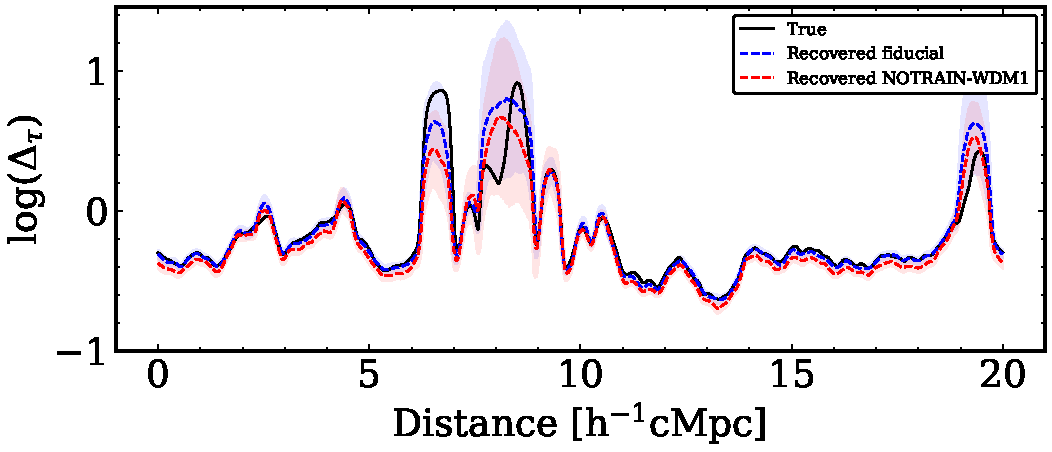
\includegraphics[width=0.9\linewidth]{img/ML/skewer_notrain_wdm1.pdf}
    \caption{The \texttt{NOTRAIN-WDM1} model predicting on a WDM1 skewer, compared to the fiducial model trained on the whole \texttt{SHERWOOD} dataset.}
    \label{fig: skewer notrain wdm1}
\end{figure}

\begin{figure}
    \centering
    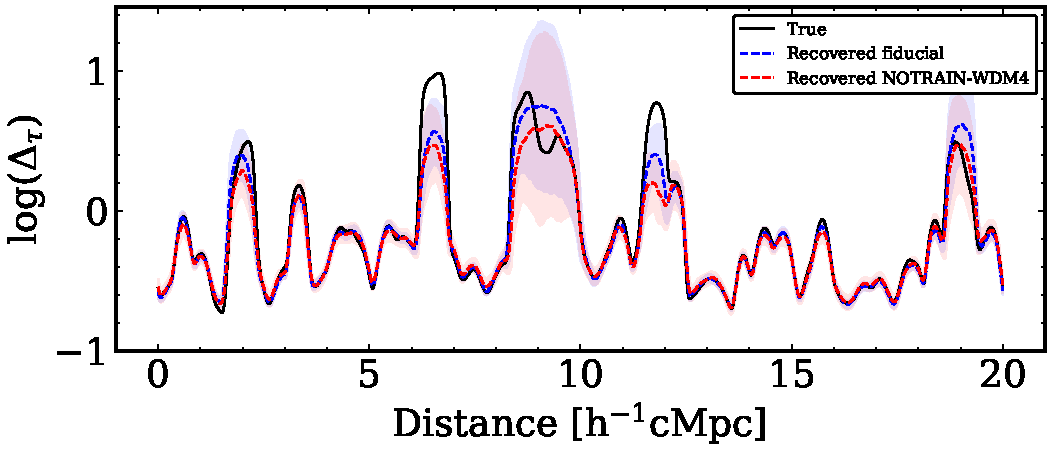
\includegraphics[width=0.9\linewidth]{img/ML/skewer_notrain_wdm4.pdf}
    \caption{The \texttt{NOTRAIN-WDM4} model predicting on a WDM4 skewer, compared to the fiducial model trained on the whole \texttt{SHERWOOD} dataset.}
    \label{fig: skewer notrain wdm4}
\end{figure}
Note the clear covariate shift effect in Figure \ref{fig: skewer notrain wdm1}, where the \texttt{NOTRAIN-WDM1} have a systeatic bias towards lower densities. In comparison, in Figure \ref{fig: skewer notrain wdm4} the model \texttt{NOTRAIN-WDM1} shows no clear indication of any bias, and is almost indistinguishable from the fiducial model. In the former case, the model has to extrapolate on data generated from an unseen model, which gives clearly an incorrect predidction. In the later case, the model has been trained on CDM and WDM3, so predicting on WDM4 is an interpolation task.

\subsection{Extreme covariate shift and malicious data}
In regression tasks related to computer vision, it is customary to mask certain parts of the input to explore how the model reacts to specific features. Following this idea, we have designed a set of malicious Lyman-$\alpha$ skewers that include artefacts and unnatural features that are not present in the training dataset. Therefore, this can be considered as an extreme case of cavoariate shift. In Figure \ref{fig: skewer malicious} we show the fiducial model predictions for two such skewers. In the first case, we consider a fully saturated skewer with zero flux and only a small amount of noise. Observe how the model makes an educated guess and predicts the mean density for the whole skewer. However, the model is very confident in the predictions and produces minimal uncertainties. This is not correct from the physical standpoint, since any density higher that the truth can produce a saturated flux. In the second skewer we have complete transmission except a saturated absorption feature. The predictions for the pixels with complete transmissions are below the mean density, and on the saturated pixels it is above the mean density with a higher uncertainty. This is closer to a ``real'' absorption feature with more accurate prediction.

\begin{figure}
    \centering
    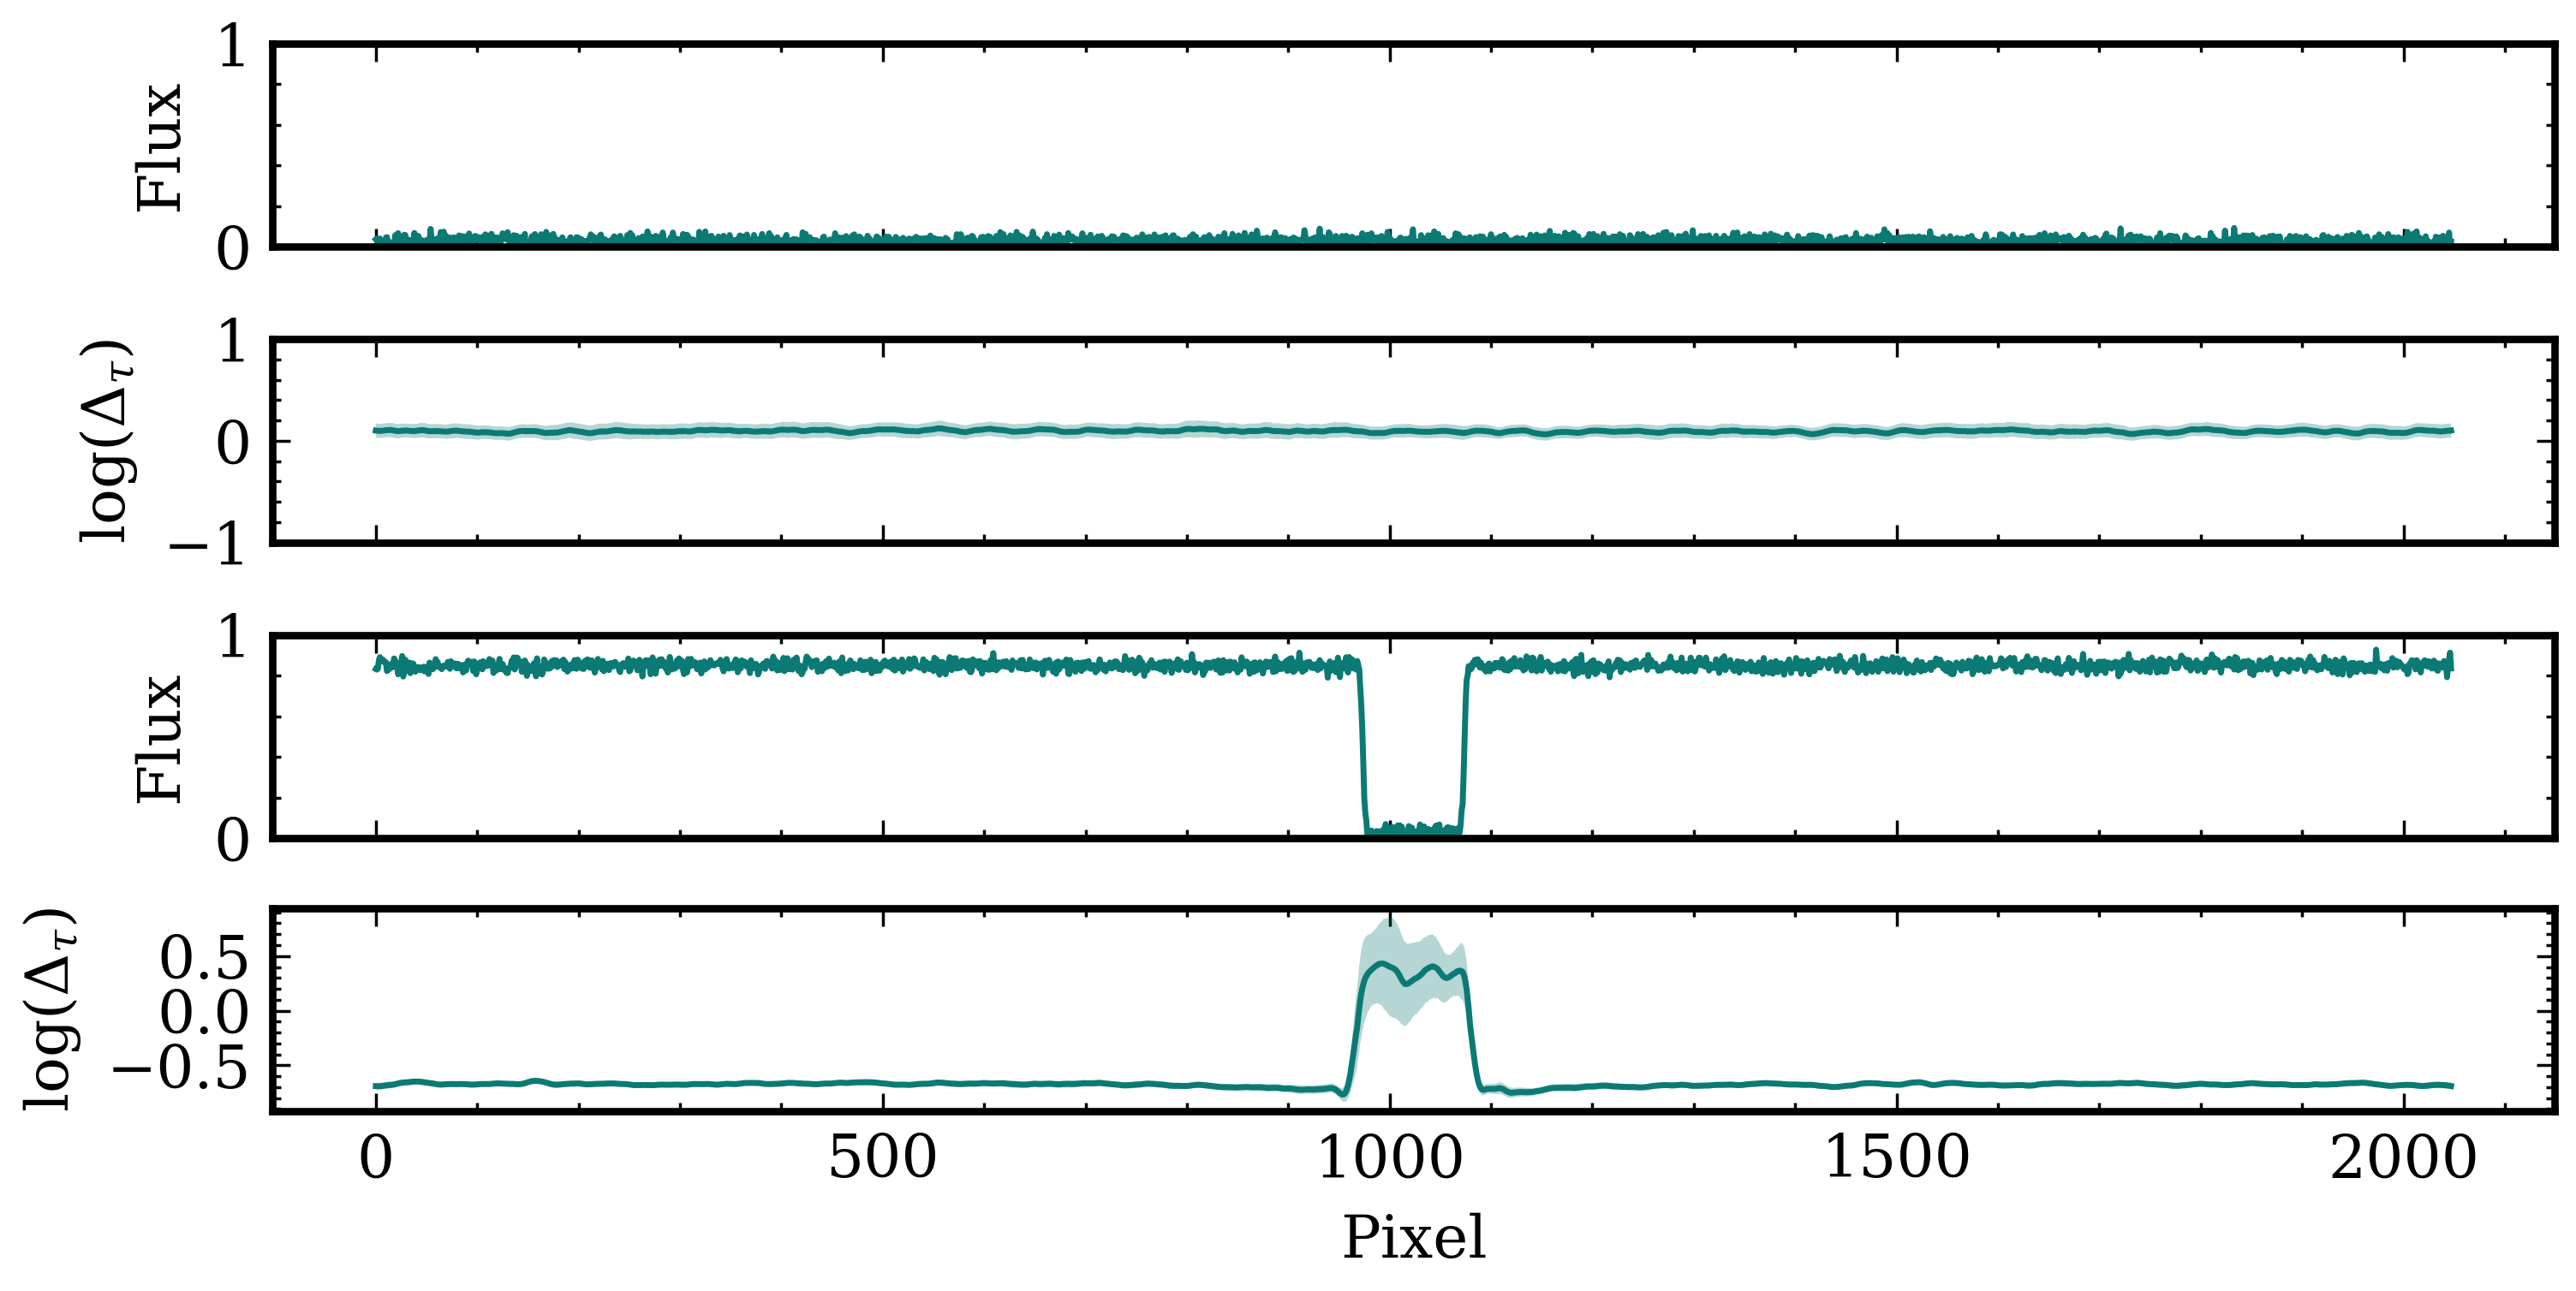
\includegraphics[width=0.9\linewidth]{img/ML/malicious_input.png}
    \caption{The \texttt{NOTRAIN-WDM4} model predicting on a WDM4 skewer, compared to the fiducial model trained on the whole \texttt{SHERWOOD} dataset.}
    \label{fig: skewer malicious}
\end{figure}


\subsection{Model pruning}
Prunning refers to the idea of eliminating certain components of a deep neural network, or equivalently, considering a sub-network. The motivation to prune a network is generally to reduce the number of parameters, which can improve interpretability, and allow users to better trace the flow of information through the network. Since most deep network are over-parametrised, pruning can improve training while mantaining a very similar performance to the original architecure. Pruning is an active area of research, and there are efforts being made to use domain-specific expertise to prune networks and make informed choices about their topology \cite{pruning}. In this work, we have used \texttt{OPTUNA} in section \ref{sec:optuna} to tune the hyperparameters of the model on the sole basis of a performance metric function. This naturally over-parametrises the network, with connections and filters that might be redundant. This means that there is a potential room for improvement when it comes to finding more interpretable networks with fewer parameters and a more stable trainig.

To illustrate how pruning can affect the performance of our model, we briefly focus on the first convolutional layer of the architecutre in Figure \ref{fig:ML nn architecture}. In Figure \ref{fig: filter acti} we show the activation of the first 4 convolutional filters for a trained network with architecute [2, 2], [4, 16] for a randomly selected skewer, following the notation in Table \ref{table: fiducial architecture}. Note that out of the four filters, the blue and green ones are scaled versions of each other, and similarly, the red and orange filters are also scaled versions of one another. To test of this redundancy affects the network, the prune half of the filters in this first layer to an architecture [2, 2], [2, 16]. Figure \ref{fig: pruned NLL} shows the training NLL curve for both architecures. As can be seen, they reach a simialar performace in terms of the NLL, but the pruned architecure has a more stable learning curve and convergence in a smoother way.


\begin{figure}
    \centering
    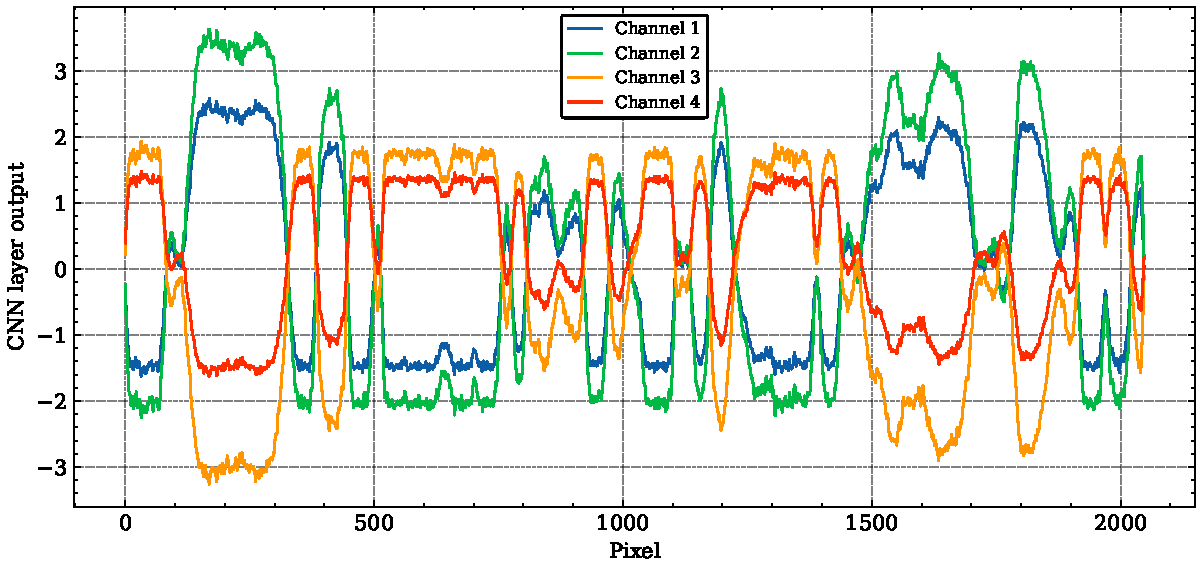
\includegraphics[width=0.9\linewidth]{img/ML/filter-acti.pdf}
    \caption{First layer activation of the convolutional filters for a trained network with architecture [2, 2], [4, 16] for a randomly selected CDM skewer from \texttt{SHERWOOD}.}
    \label{fig: filter acti}
\end{figure}

\begin{figure}
    \centering
    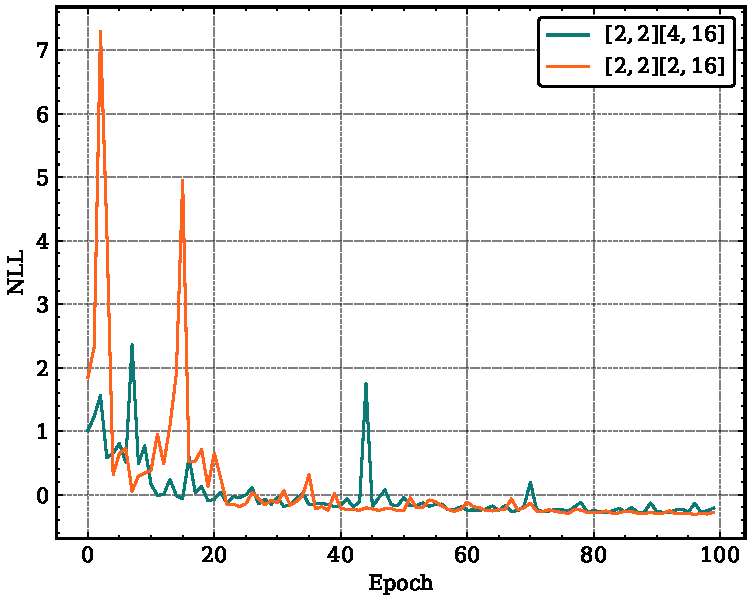
\includegraphics[width=0.9\linewidth]{img/ML/NLL_diff_channels.pdf}
    \caption{Training curves for the NLL comparing the model [2, 2], [4, 16] and the prunned architecutre [2, 2], [2, 16] with half of the convolutional filters in the first layer.}
    \label{fig: pruned NLL}
\end{figure}